\documentclass[a4paper,12pt]{report}

\usepackage{alltt, fancyvrb, url}
\usepackage{graphicx}
\usepackage[utf8]{inputenc}
\usepackage{float}
\usepackage{hyperref}
\usepackage{xurl}

\usepackage[italian]{babel}
\usepackage[italian]{cleveref}
\usepackage[toc,page]{appendix}


\title{Relazione Progetto OOP 2022}
\author{
    Stefano Furi\\
    Luca Rapolla\\
    Michele Montesi\\
    Ezmiron Deniku\\
}
\date{\today}

\begin{document}

\maketitle

\tableofcontents

\chapter{Analisi}
\section{Requisiti}
Il software costruito mira all'emulazione del \emph{Retro Game} Pang. Con Retro Game si intende un gioco di una precedente generazione, il quale necessita di un emulatore per essere giocato al giorno d'oggi, in quanto difficilmente reperibile in forma fisica. 
\subsubsection{Requisiti Funzionali}
Il gioco è composto da tre scenari principali: Menù d'inizio, sequenza di gioco e fine gioco.
\begin{itemize}
    \item Nel \emph{Menù di Inzio} è possibile scegliere il proprio \texttt{Nickname}, visualizzare la \emph{Leaderboard} locale ed avviare la sequenza di gioco.
    \item Durante Sequenza di gioco, il giocatore controlla un personaggio, il quale dovrà far scoppiare delle sfere (ognuna sdoppiabile per tre volte) tramite l'utilizzo di un arma. Una volta finite le sfere, il giocatore passa al prossimo stage, dove la difficoltà aumenta. Durante la sessione di gioco, compare (ad intervalli randomici) un nemico il quale, planando verso un punto specifico, potrebbe colpire il personaggio principale. Vengono inoltre generati dei bonus che, se raccolti dal personaggio, incrementano il punteggio della partita corrente. Insieme a questi ultimi, nello stage di gioco possono comparire anche PowerUp, che hanno lo scopo di modificare lo stato attuale del gioco. Ogni volta che il personaggio viene colpito, viene decurtata una vita.
    \item Al termine delle tre vite, si passa alla fine del gioco dove il punteggio viene salvato nella \emph{Leaderboard} e viene chiesto all'utente se si desidera effettuare una nuova partita, oppure abbandonare l'applicazione.
\end{itemize}

\subsubsection{Requisiti non funzionali}
In quanto RetroGame, il gioco deve poter funzionare anche su architetture a basse prestazioni.

\section{Analisi e modello del dominio}
Il software dovrà essere in grado di generare degli stage di difficoltà sequenziale. La difficoltà è determinata dal numero e dalla velocità delle sfere presenti nello stage di gioco. Ogni sfera si muove nello spazio rimbalzando sul terreno e sui bordi e ogni sfera ha la caratteristica di essere duplicabile nel caso in cui venga colpita da un proiettile. Con duplicazione si intende il passaggio da uno stato padre ad uno figlio, eseguibile per un massimo di due volte; in totale quindi tre stati (Padre-Figlio-Nipote). L'arma assegnata al personaggio prinicpale è un arpione il quale, a seconda del \emph{PowerUp} attivo, può assumere tre utilizzi diversi:
\begin{itemize}
    \item \emph{Arpione Classico}: il personaggio può sparare un solo arpione per volta verso l'alto, e nel momento in cui l'arpione raggiunge il limite superiore dello stage, viene riaquisito. 
    \item \emph{Arpione Appiccicoso}: il personaggio spara verso l'alto un arpione per volta il quale, nel momento in cui raggiunge il limite superiore dello stage, si "appiccica" per un determinato intervallo di tempo.
    \item\emph{Doppio Arpione}: il personaggio può sparare due arpioni per volta senza il bisogno di aspettare che il primo dei due arrivi al limite superiore dello stage.
\end{itemize}
Nello scenario è inoltre presente un uccello il quale attraversa lo stage orizzontalmente e durante la attraversata, può planare verso una determinata posizione per poi continuare il suo percorso. Anche l'uccello può essere colpito dall'arpione. 
Il giocatore ha a disposizione un certo numero di vite, le quali venogno decurtate in caso di collisione con un entità avversa. Nel momento in cui si finiscono le vite, il gioco termina e si registra il punteggio nella \emph{Leaderboard} nel caso sia abbastanza alto da superare quelli precedenti.
Lo \emph{Score} viene aumentato dall'acquisizione di Bonus che vengono generati durante la partita. Ad ogni bonus viene assegnato un punteggio diverso. Oltre ai due PowerUp che influenza l'arma, ne sono presenti altri due in grado di influire sulle sfere:
\begin{itemize}
    \item \emph{Time Freeze}: Ferma tutte le sfere attive e le riattiva dopo un certo periodo di tempo.
    \item \emph{Bomba}: Fa esplodere tutte le sfere a meno che non siano già al terzo stato (Nipote: stato più piccolo): in questo caso vengono ignorate.
\end{itemize}
A differenza dei PowerUp rivolti all'arma, gli ultimi due citati possono allo stesso tempo semplificare/peggiorare il \emph{Gameplay} del giocatore, in quanto il loro vantaggio/svantaggio varia in base al momento in cui vengono raccolti.
Gli elementi costitutivi del problema sono sintetizzati in figura \Cref{img:abstract}.

\begin{figure}[H]
\centering{}
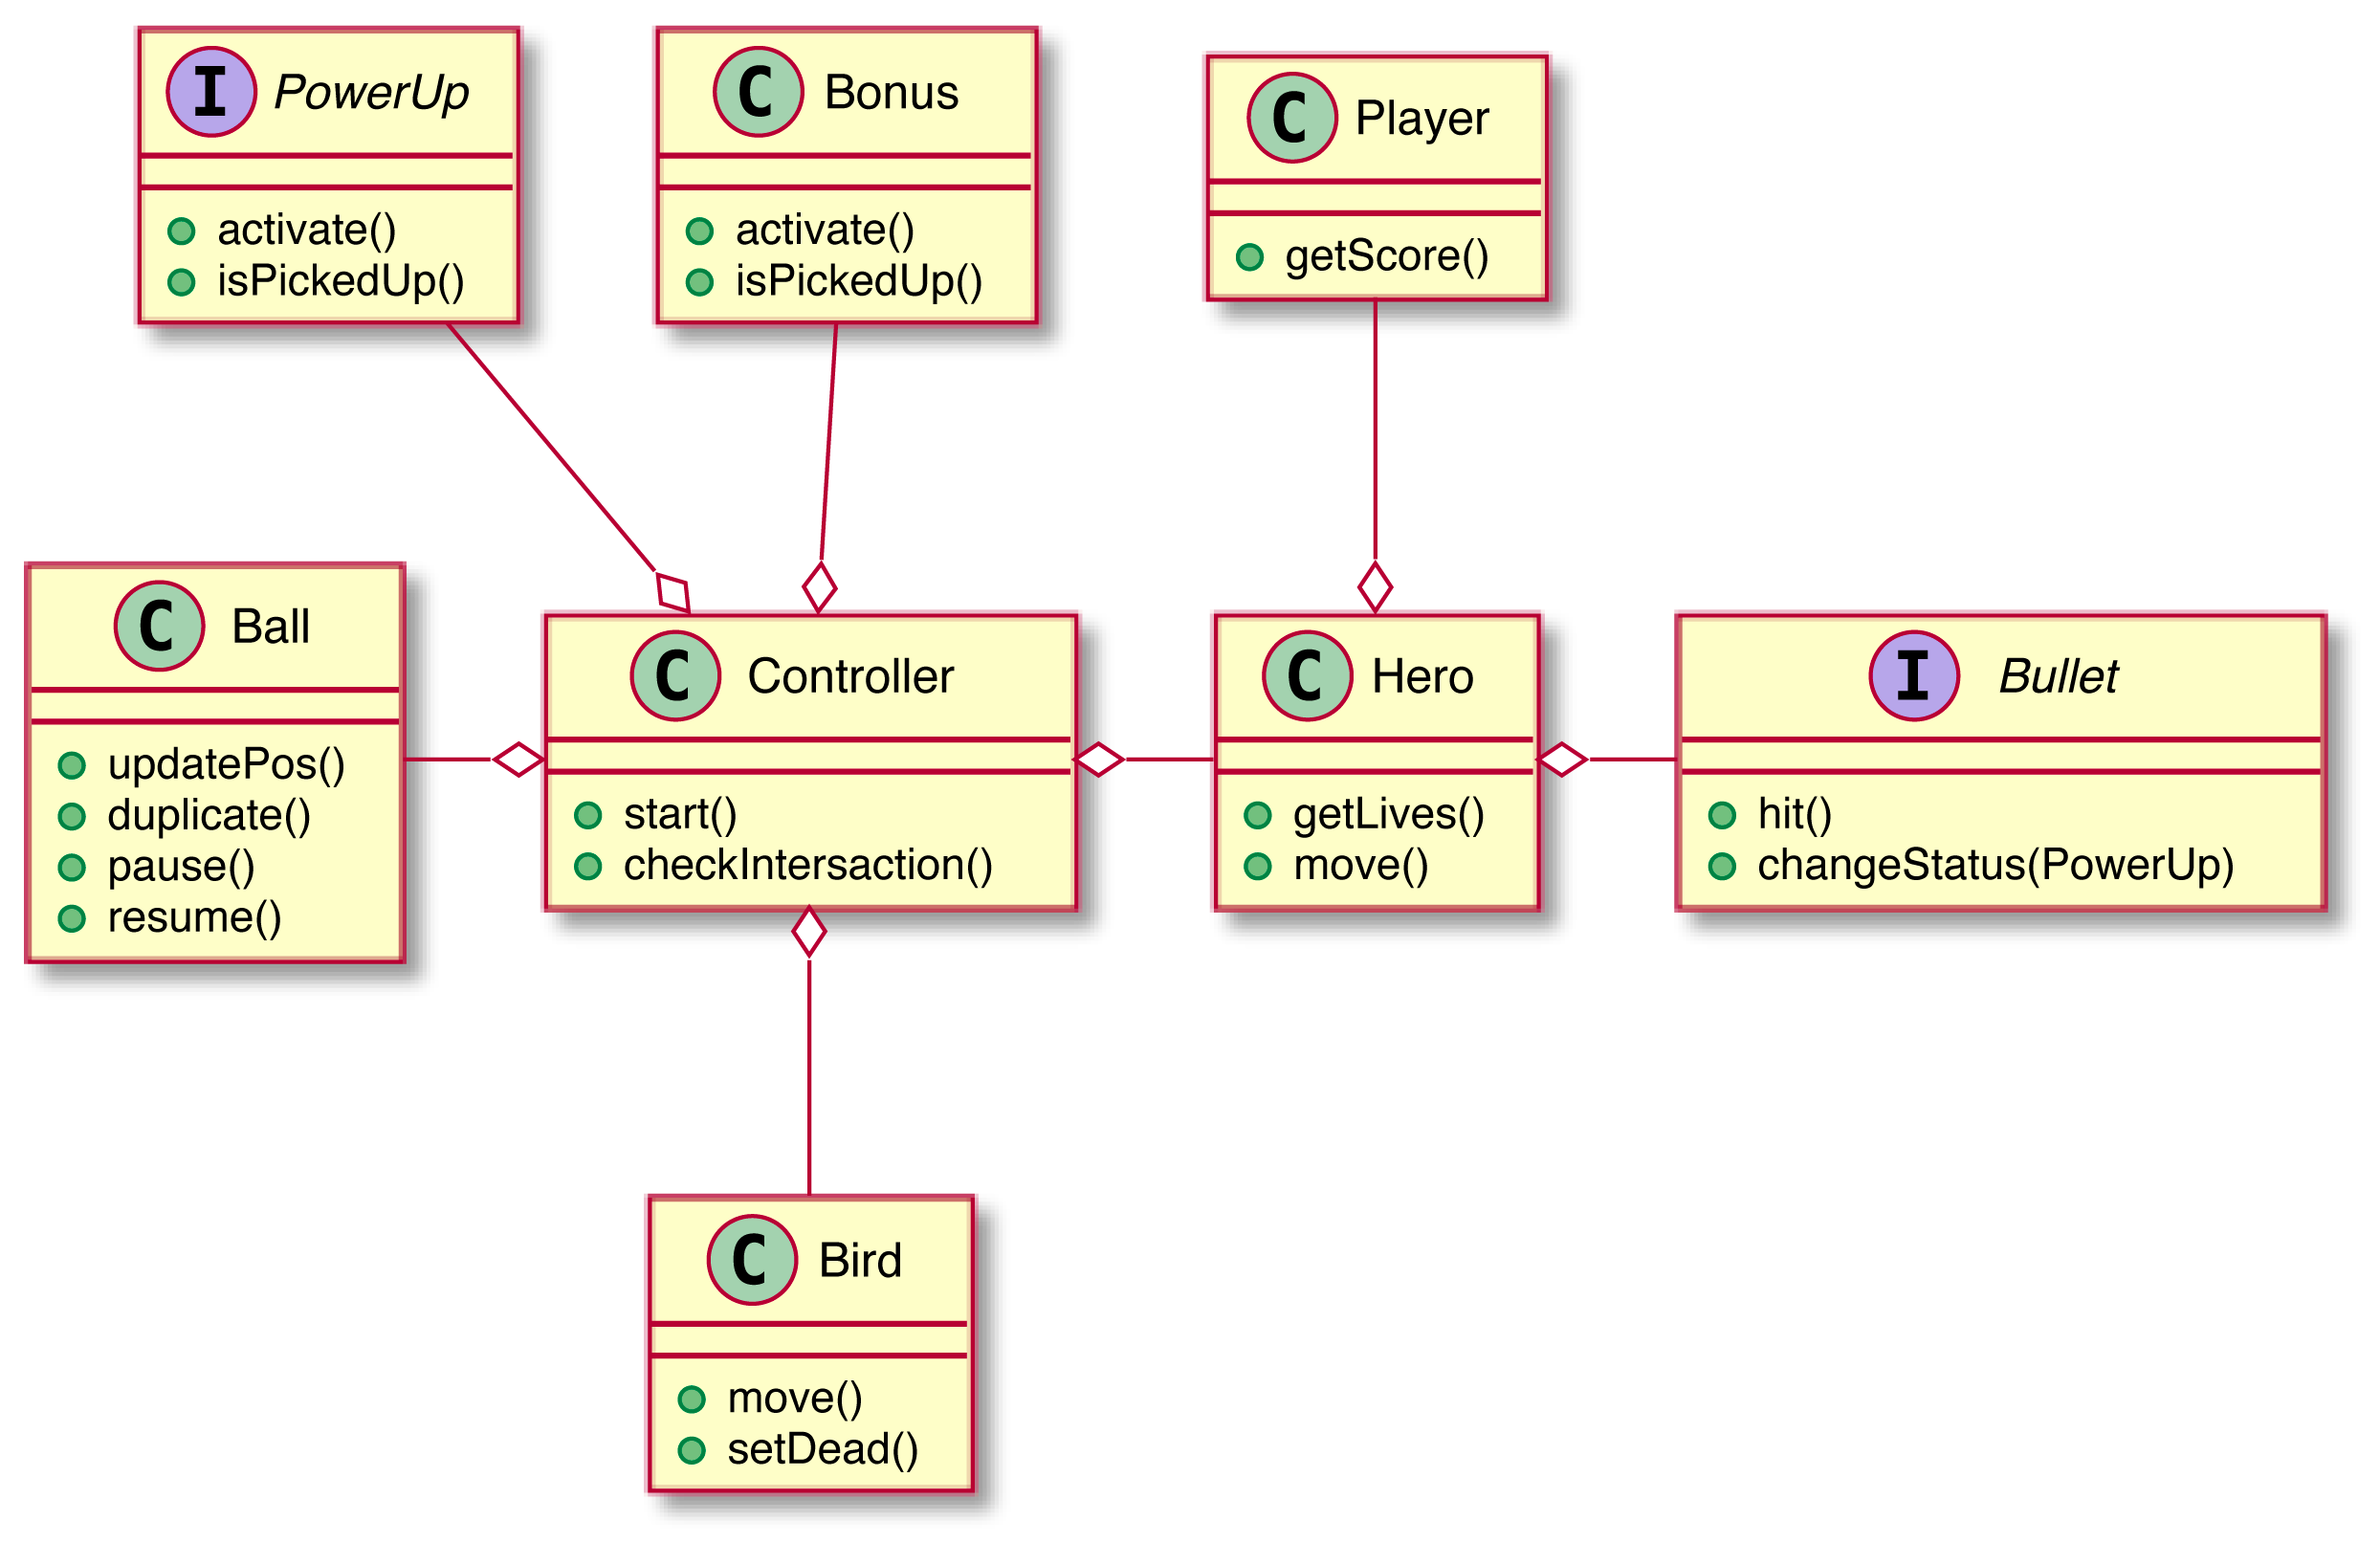
\includegraphics[width=14cm]{img/AbstractUml.png}
\caption{Rappresentazione UML del Contesto di gioco}
\label{img:abstract}
\end{figure}

\chapter{Design}
\section{Architettura}
L'architettura di Pang segue il pattern Architetturale MVC. In particolare, Pang si compone di un Controller composto da tre diversi sotto-controller i quali vengono istanziati all'interno di esso. Questi tre sono classi attive che fungono da gestori degli elementi portanti del model: 
\begin{itemize}
    \item \texttt{EntityHandler}
    \item \texttt{PickableHandler}
    \item \texttt{PauseHandler}
\end{itemize}
Il primo di essi ha lo scopo di gestire e mantenere le strutture dati di una sottoparte del model, e verificare le interazioni tra le diverse entità di quest'utilmo, per esempio, gestire le collisioni delle sfere con il personaggio. In particolare, questa classe fa uso di contenitori delle diverse entità; più nello specifico, le entità gestite sono \texttt{Ball}, \texttt{Bird}, \texttt{Arpion} e \texttt{Hero}. Queste ultime, sono le radici del model, e vengono incapsulate e gestite a loro volta da differenti \emph{Handlers}. Sommando il tutto, la classe \texttt{EntityHandler} gestisce e coordina i relativi controller attivi per ogni entità (\texttt{BallHandler}, \texttt{EntityHandler}, \texttt{Hero} e \texttt{GunBag}) e fa in modo che le interazioni tra gli elementi del model avvengano correttamente.

Il secondo di essi fornisce un controllo attivo sugli elementi \emph{Pickable} ovvero \texttt{Bonus} e \texttt{PowerUp}, e verifica se il personaggio di gioco raccoglie questi elementi.

L'ultima interfaccia invece, ha lo scopo di attivare la funzionalità della pausa durante il gioco, stoppando momentaneamente l'esecuzione dei controller degli elementi fondamentali del dominio.

Infine l'entry point della View è definito da \texttt{Visual}, una classe che ha il compito di ricevere costantemente posizioni aggiornate e "avvisare" la \emph{GUI} che è si è verificato un cambiamento nel model, ed è quindi necessario un aggiornamento dell'interfaccia grafica. Questo permette di poter sostituire in blocco la parte di View, in quanto \texttt{Visual} e \texttt{Controller} lavorano indipendentemente dalla libreria grafica utilizzata.

\begin{figure}[H]
\centering{}
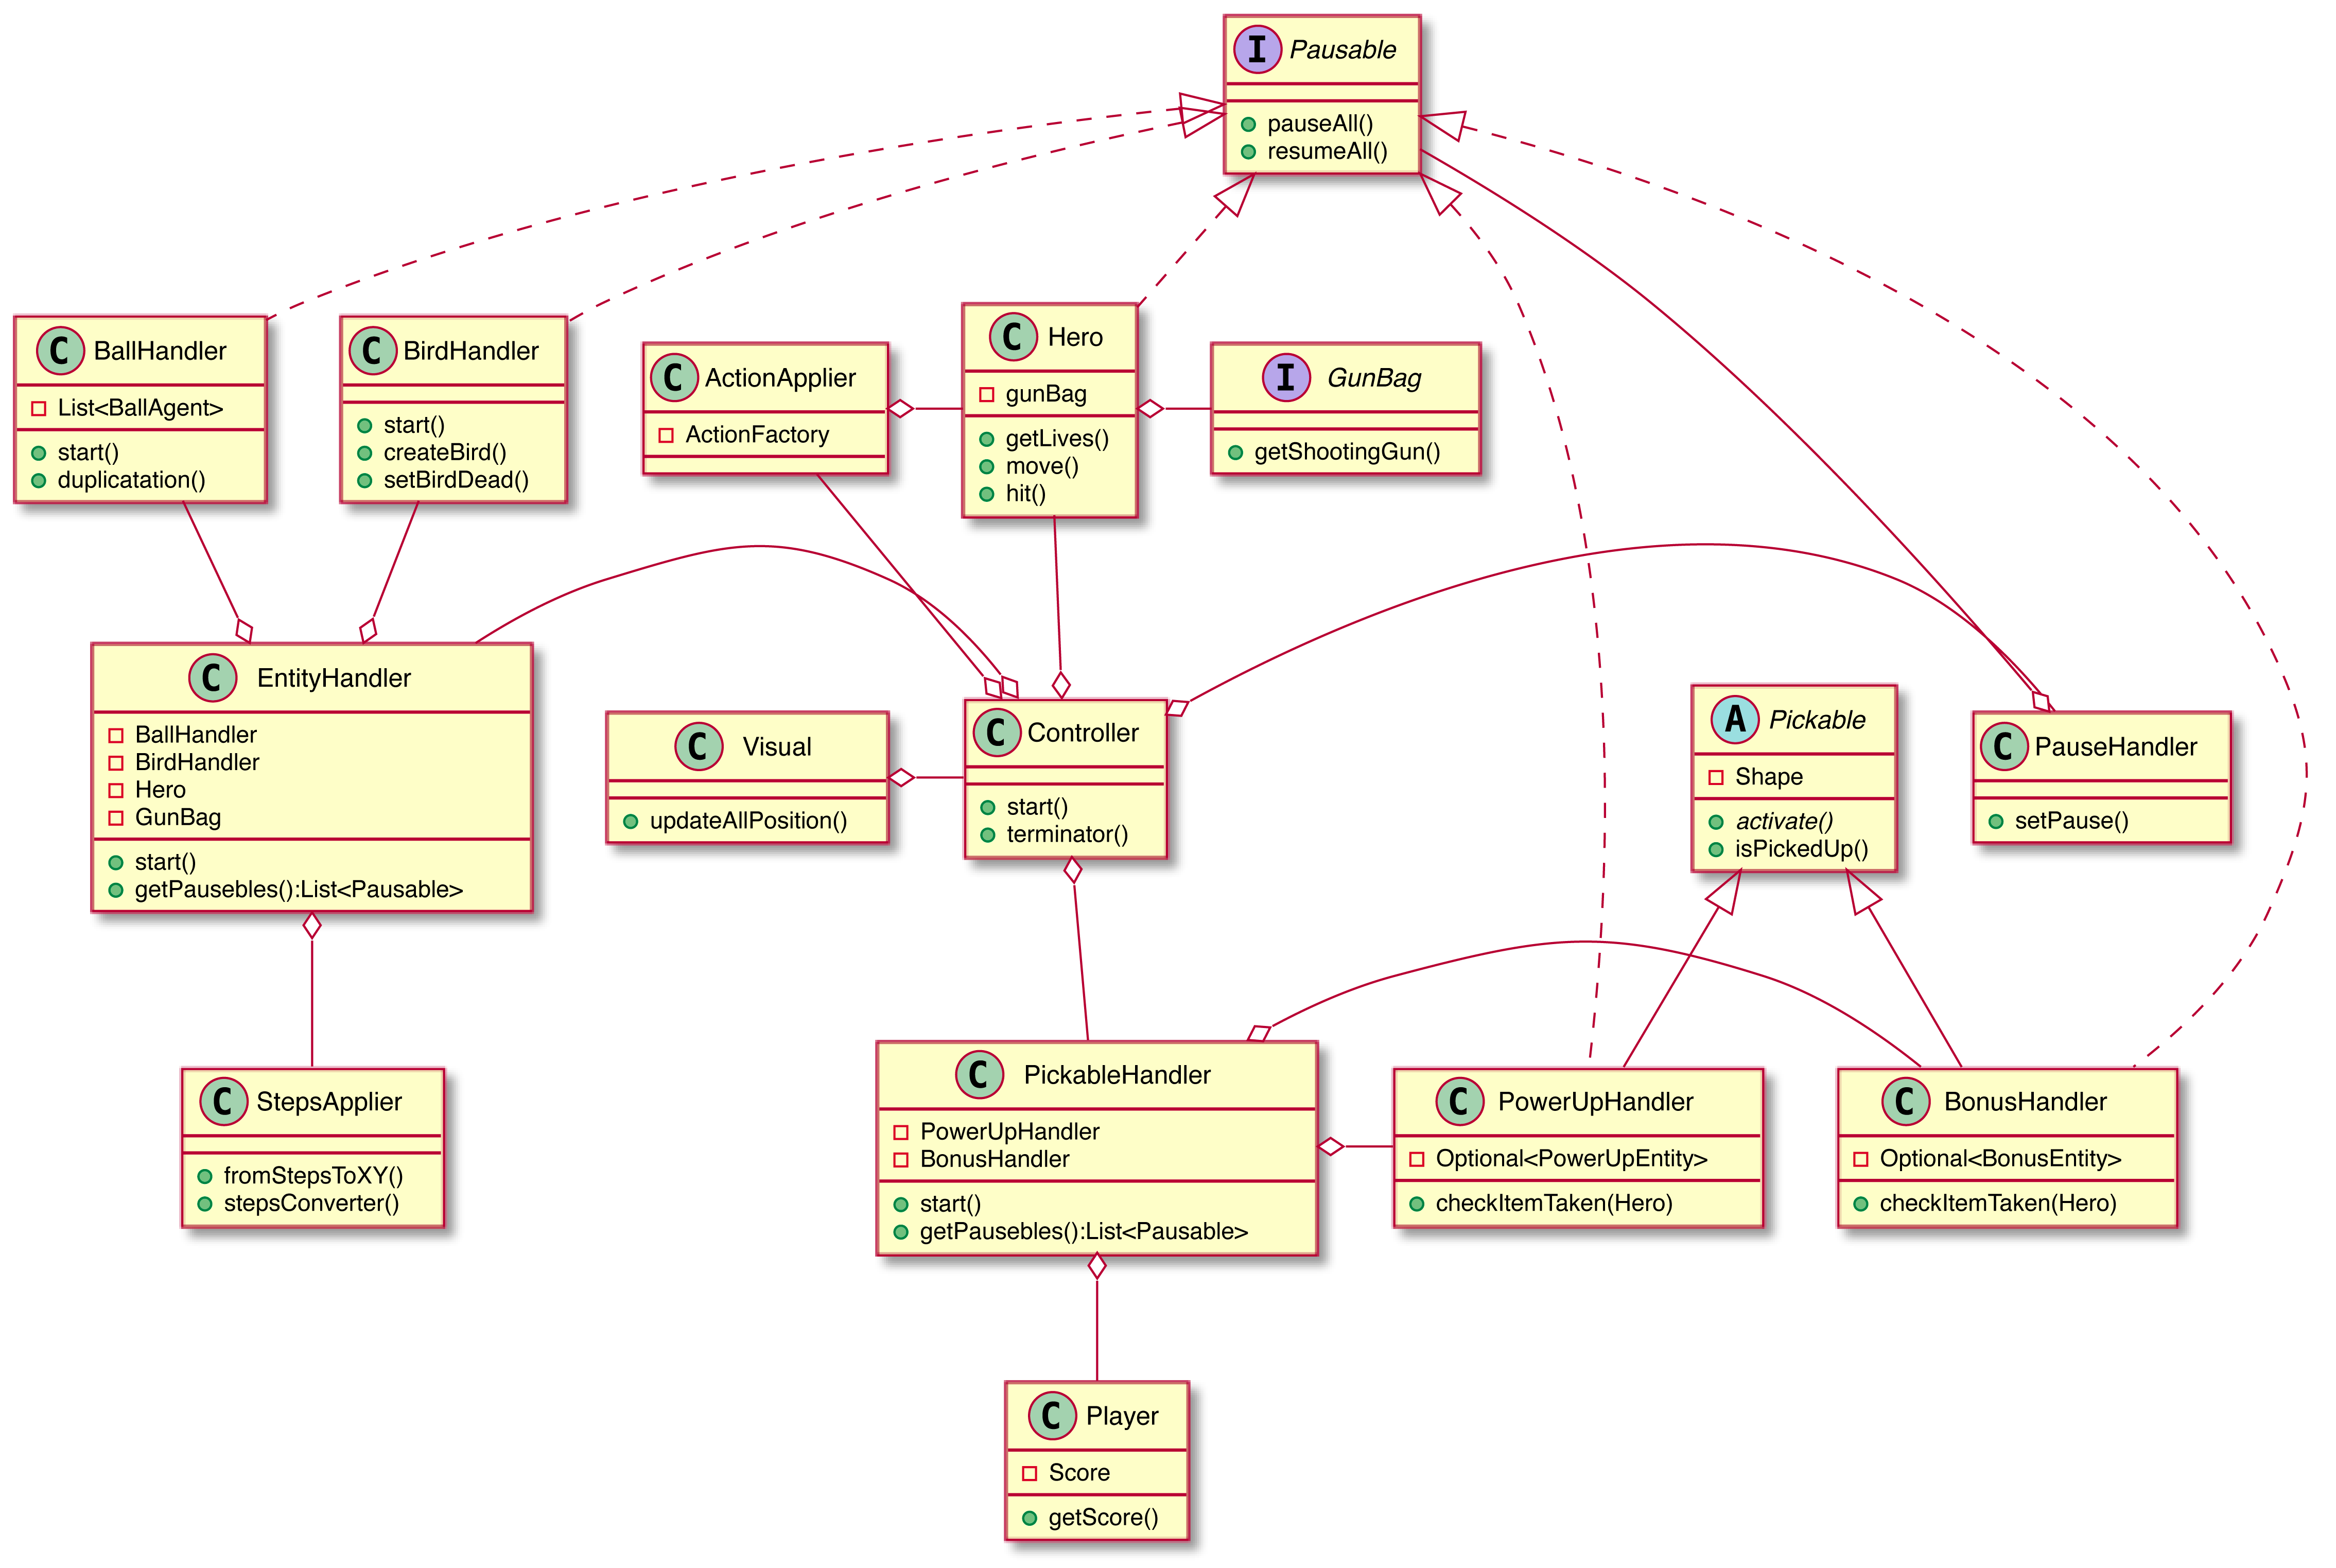
\includegraphics[width=16cm]{img/All.png}
\caption{Rappresentazione UML di MVC, al centro \texttt{Controller} definisce l'entry point di tutti i sotto-controller e \texttt{Visual} permette di comunicare con la view indipentemente dalla libreria grafica implementata}
\end{figure}

\section{Design Dettagliato}
\subsection{Stefano Furi}
\subsubsection{Gestione delle sfere e cambiamento del loro stato}

\begin{figure}[H]
\centering{}
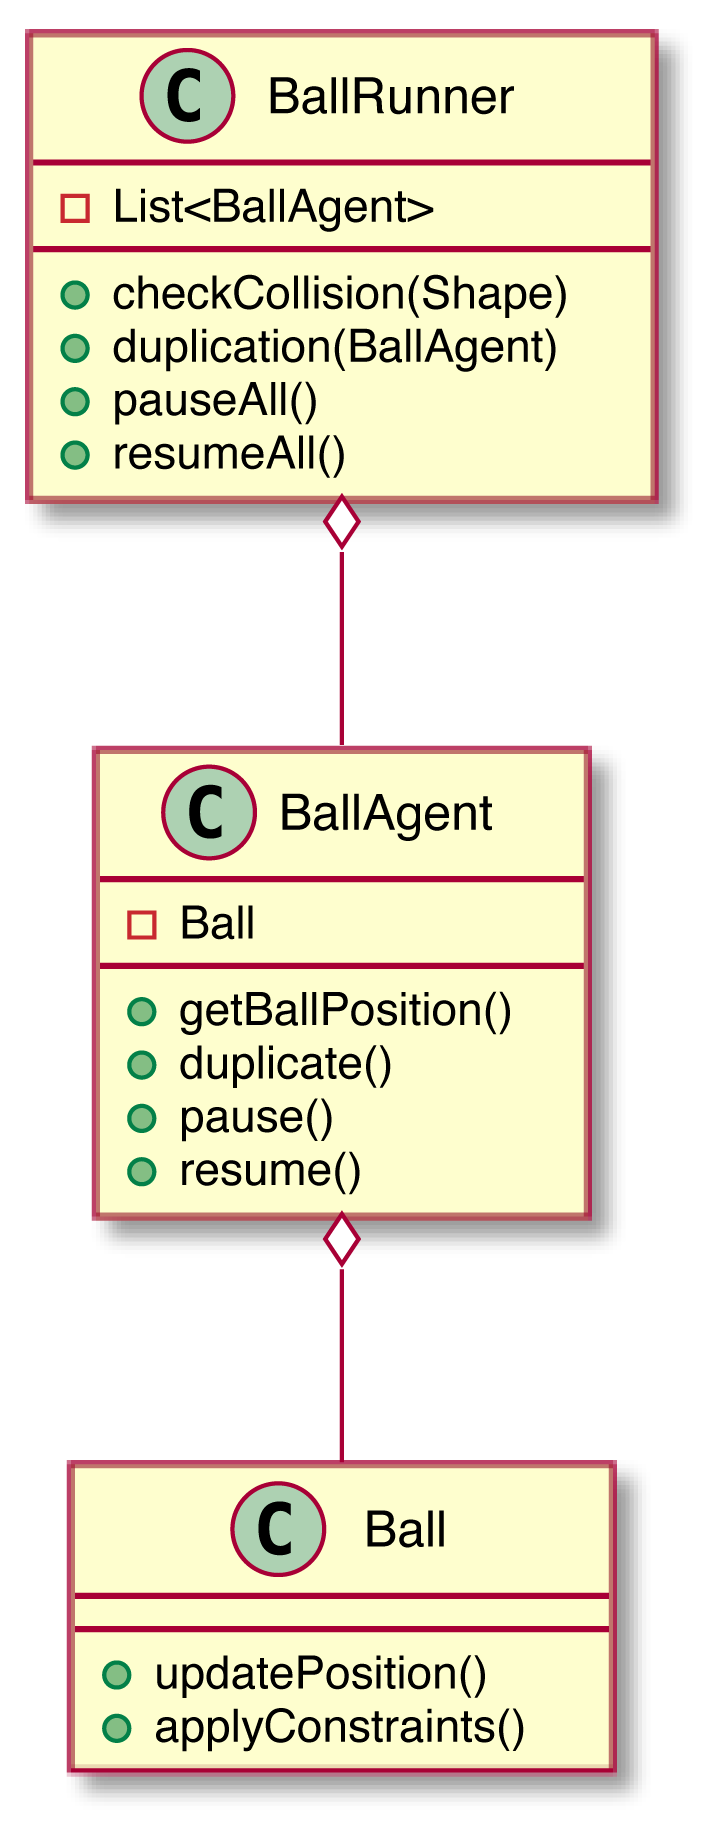
\includegraphics[width=3cm]{img/BallWrapping.png}
\caption{Rappresentazione UML della gestione delle Sfere}
\end{figure}

\paragraph{Problema:} Pang deve essere in grado di gestire e cambiare lo stato (anche contemporaneamente) di tutte le sfere presenti in gioco in modo trasparente al client.
\paragraph{Soluzione:} Il concetto più a basso livello della sfera \texttt{Ball} (struttura dati che mantiene elementi come velocità, angolo della curva, posizioni, ...) viene "wrappato" all'interno di un agente \texttt{BallAgent} (Thread), il quale ad ogni sua iterazione, aggiorna la posizione della sfera che mantiene all'interno di esso. Ogni sfera è quindi wrappata all'interno di un agente, i quali a loro volta, vengono mantenuti all'interno di un "Controller" \texttt{BallRunner} che gestisce le eventuali collisioni (contro un muro/pavimento, o contro un \emph{Shape}(Arpione o Personaggio)), ed espone all'esterno i metodi di duplicazione delle, di pausa e di ripresa del movimento delle sfere.

\subsubsection{Creazione di diversi tipi di sfera con comportamento differente}

\begin{figure}[H]
\centering{}
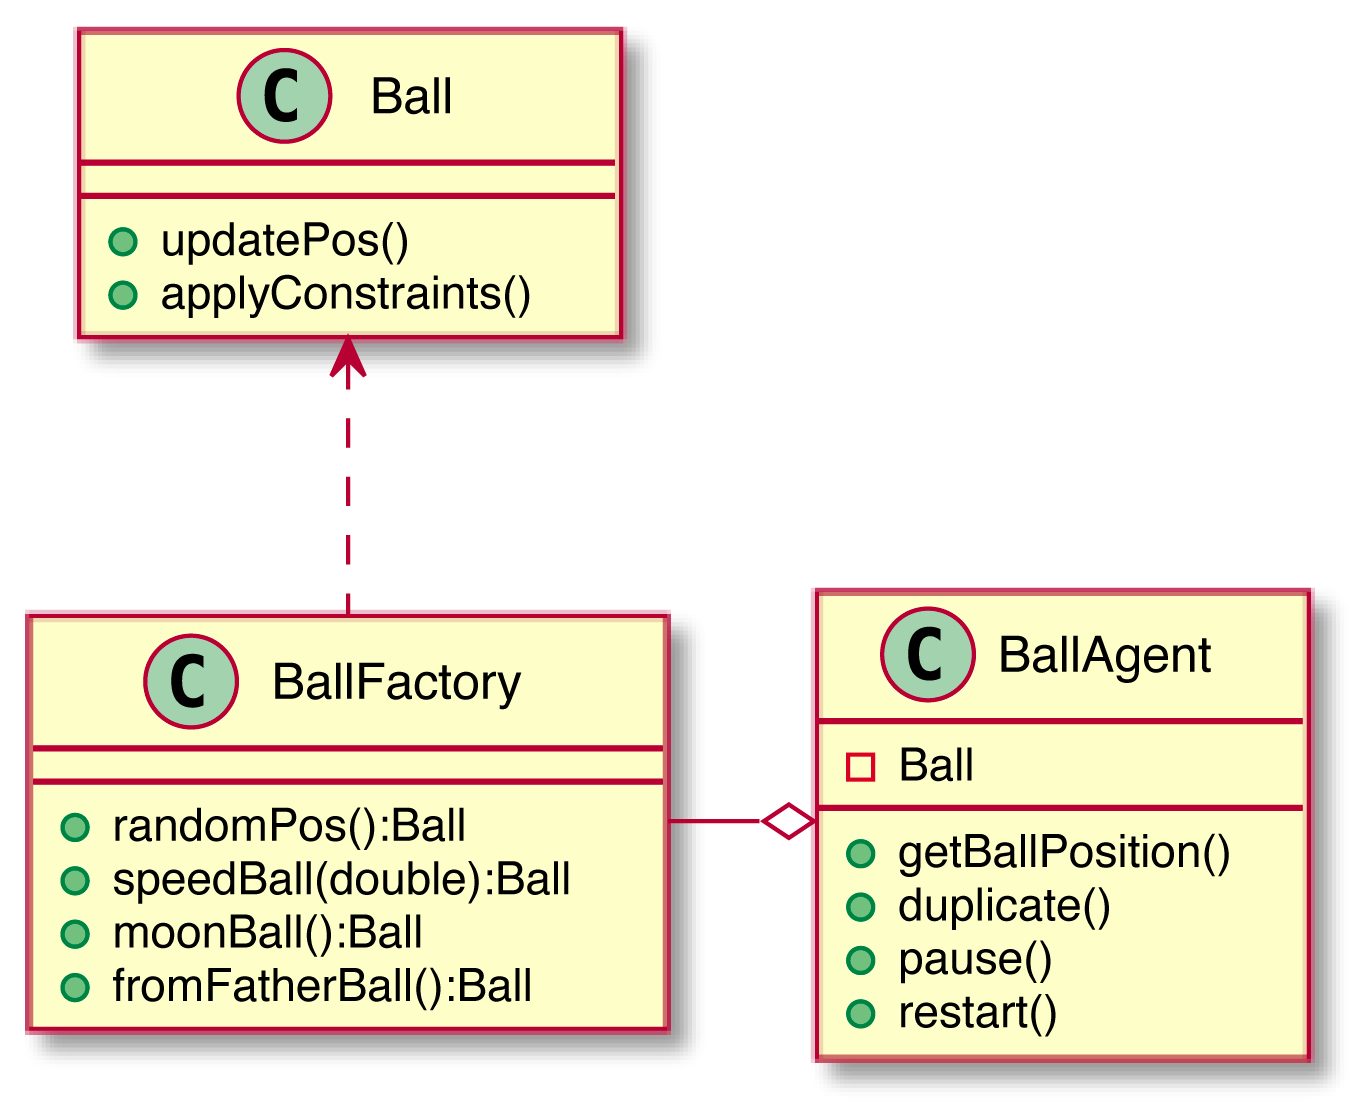
\includegraphics[width=6cm]{img/BallFactory.png}
\caption{Rappresentazione UML del pattern Factory per la creazione di diverse sfere}
\end{figure}

\paragraph{Problema:} In vista di Stage di gioco differenti e la continua creazione di nuove sfere successivamente ad una duplicazione, è necessario creare sfere con diverse proprietà e comportamenti. Questo provoca a una ripetizione continua nell'istanziazione di nuove sfere, e inoltre non rende il codice flessibile per future funzionalità aggiuntive.


\paragraph{Soluzione:} Per la creazione di diversi tipi di sfera (sfere più lente, più veloci, con dimensioni diverse,...), è risultato ottimale l'utilizzo del pattern Factory, in quanto permette di istanziare in una classe separata tutti tipi di costruzioni per le sfere. Inoltre permette di fornire metodi funzionali per le sfere (degno di nota è \texttt{fromFatherBall()}, il quale risulta molto pratico durante la fase di duplicazione di una sfera). Il fatto di utilizzare la Factory per la creazione, aiuta l'estendibilità dell'applicazione, in quanto se si volesse implementare, per esempio, uno stage in base alla difficoltà, basterà creare una sfera tramite il metodo \texttt{speedBall()} che riceve un parametro in ingresso capace di definire la velocità della palla, e quindi, la difficoltà di evitarla.



\subsubsection{Pickable: PowerUp e Bonus}
\begin{figure}[H]
\centering{}
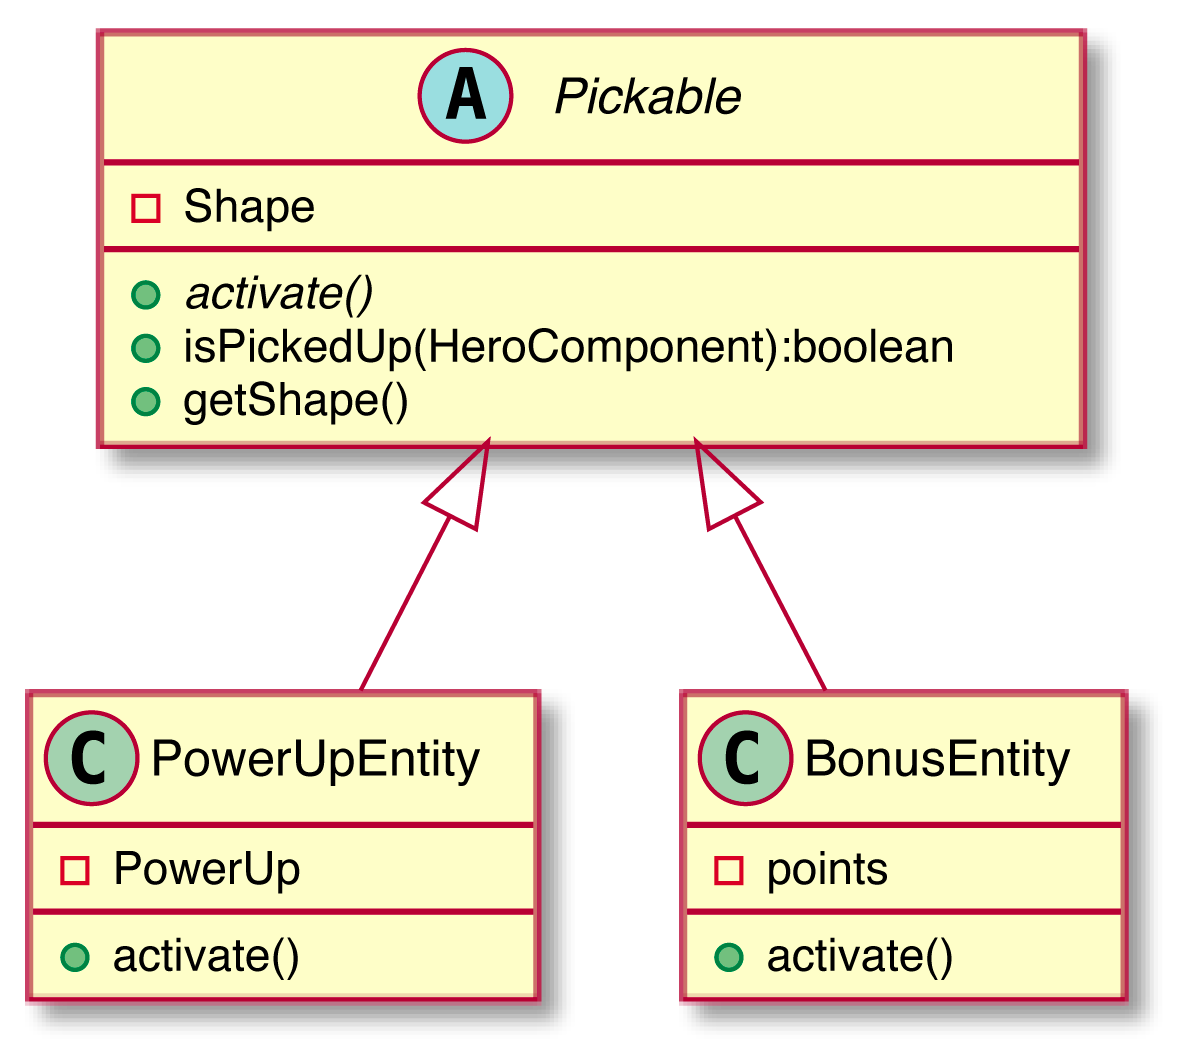
\includegraphics[width=4cm]{img/Pickable.png}
\caption{Rappresentazione UML di Template Method per PowerUp e Bonus}
\label{img:pickable}
\end{figure}

\paragraph{Problema:} l'applicativo Pang richiede la generazione casuale di PowerUp per modifcare lo stato delle sfere/arpioni, e di Bonus per incrementare il punteggio del giocatore.
Durante lo sviluppo, ci siamo accorti che queste entità condividevano molto del loro comportamento e struttura interna e stavano portando ad avere codice duplicato o ripetitivo.

\paragraph{Soluzione:} Siccome le due classi differiscono solo per qualche comportamento, tramite il pattern \emph{Template Method}, è stato possibile definire il tipo \texttt{Pickable}, il quale definisce le azioni e i comportamenti basilari di un item, per poi essere specializzato in base alle esigenze di un item.

\subsubsection{Gestione dei diversi PowerUp ed estendibilità}
\begin{figure}[H]
\centering{}
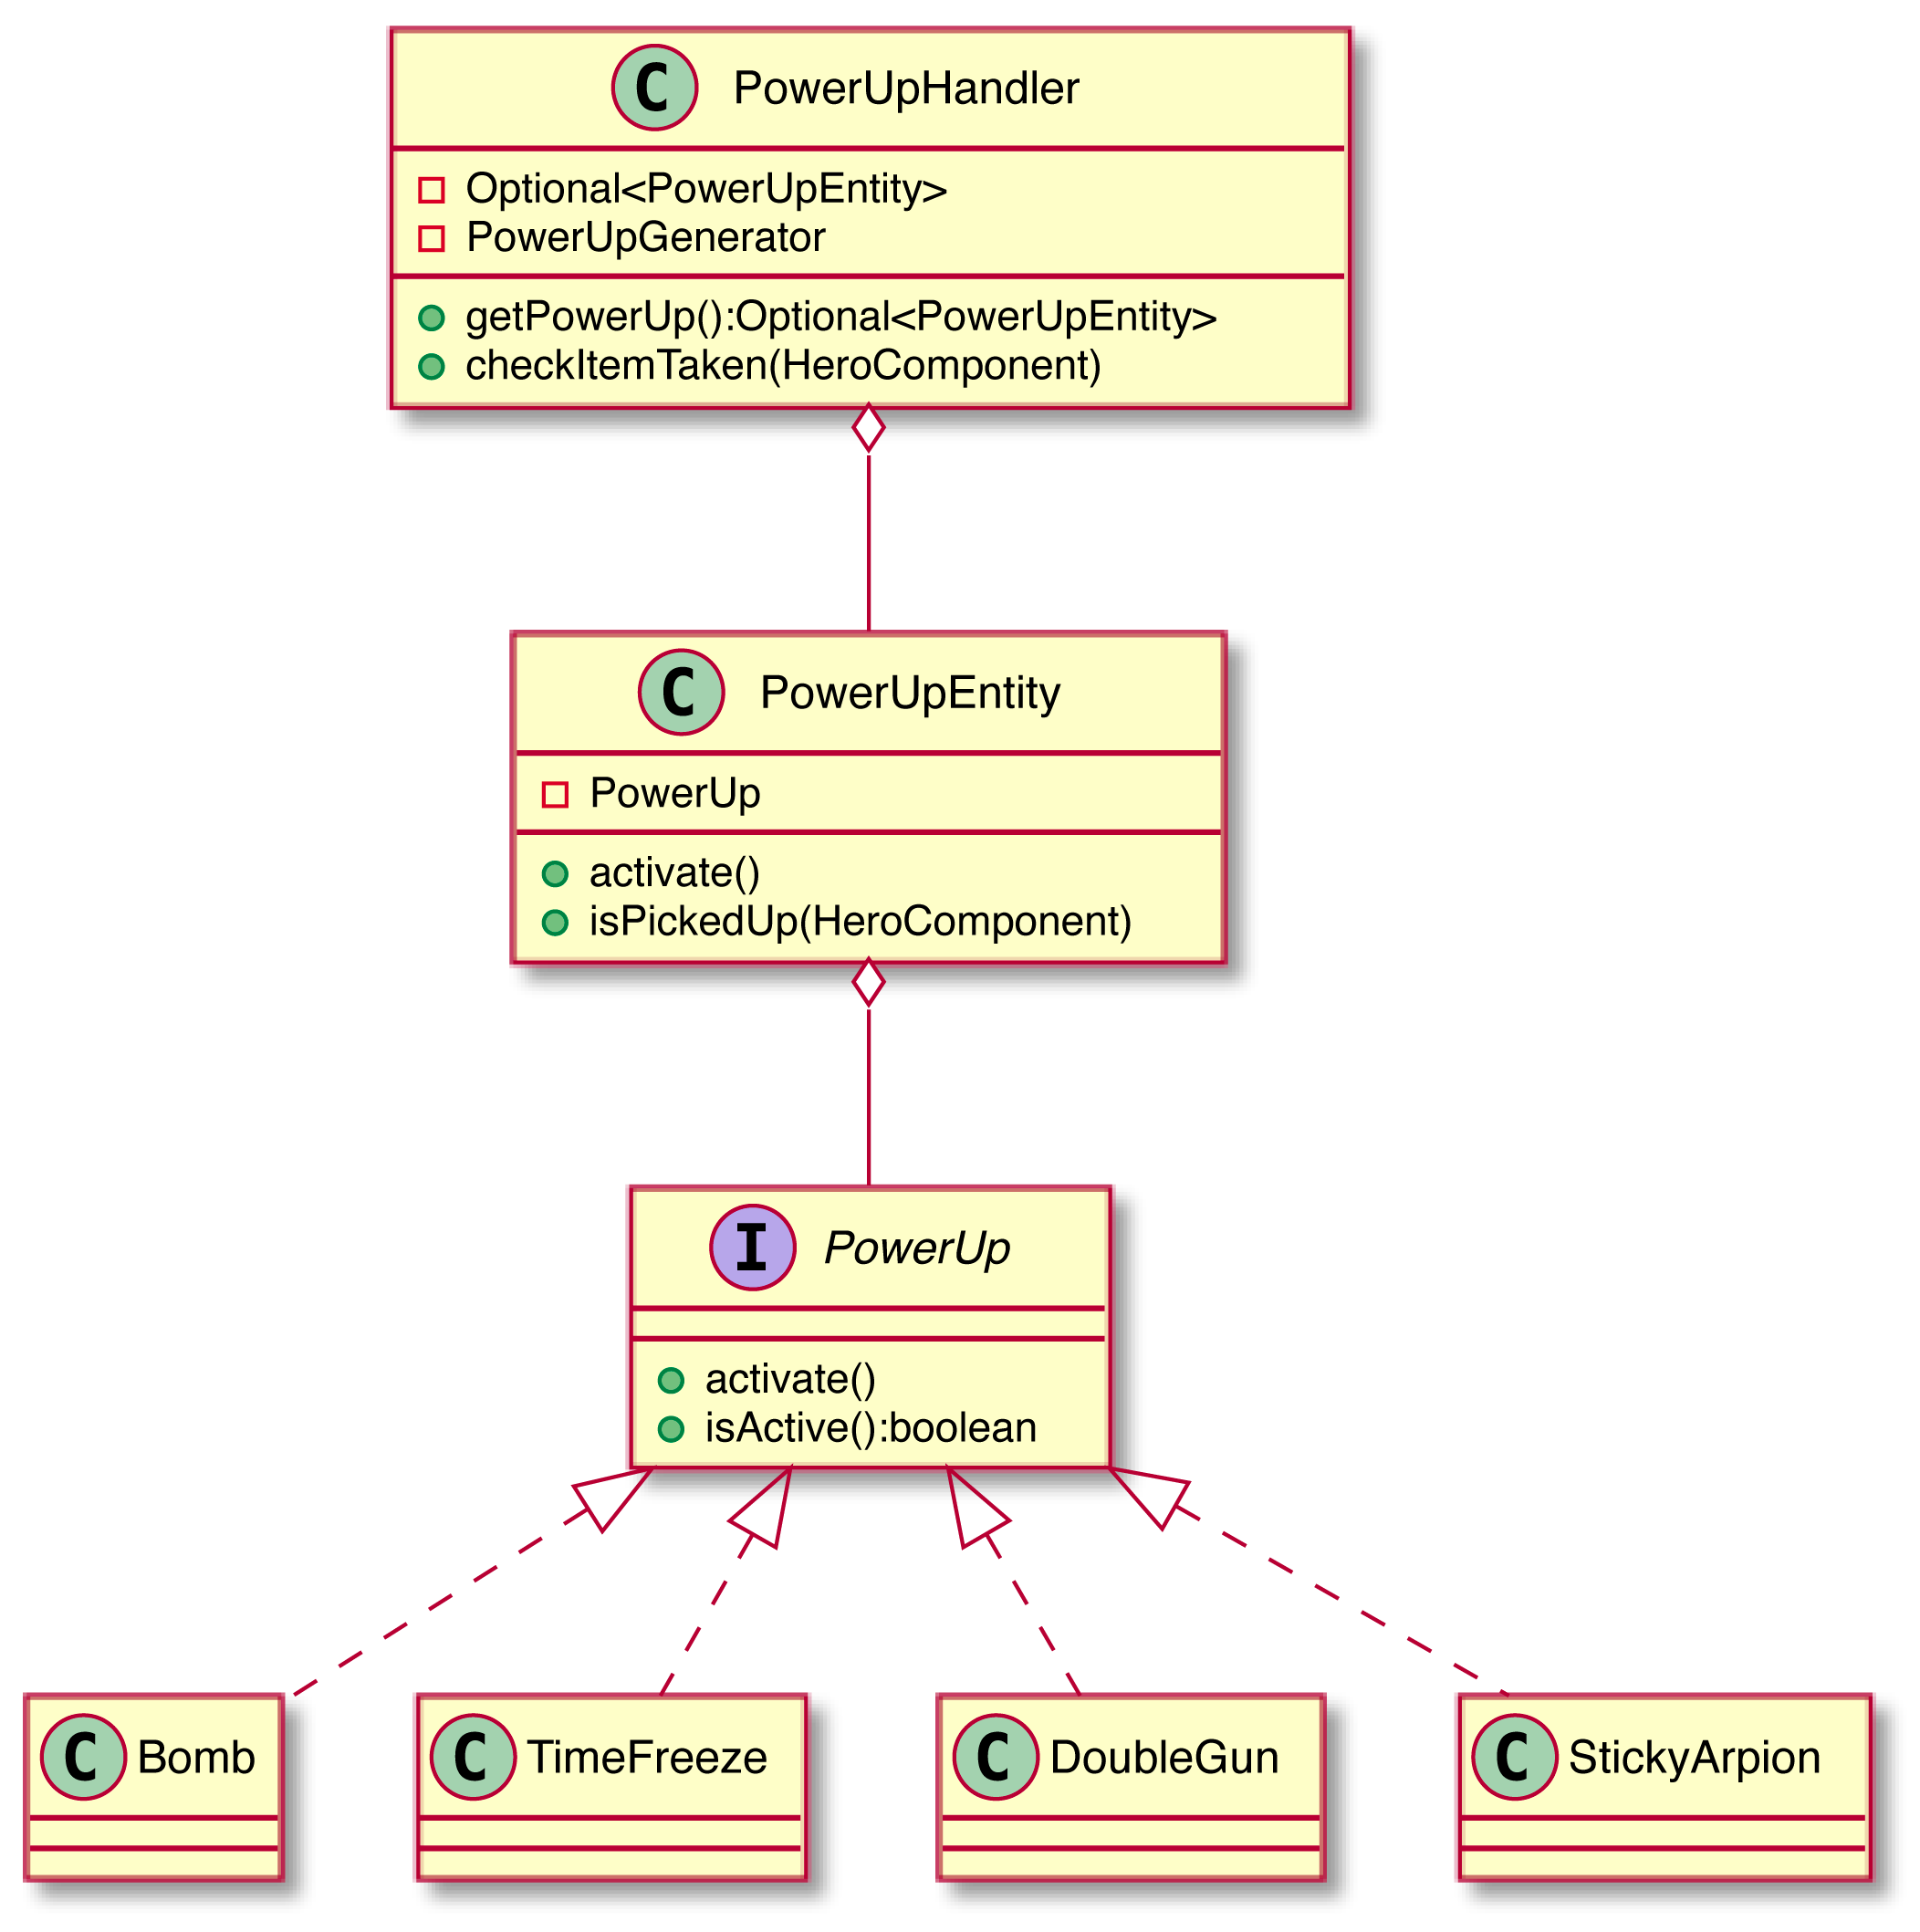
\includegraphics[width=7cm]{img/PowerUpStructure.png}
\caption{Rappresentazione UML della gestione di diversi PowerUp}
\end{figure}

\paragraph{Problema:} l'applicazione deve essere in grado di fornire un certo numero di \texttt{PowerUp}, ognuno con effetti sensibilmente diversi, ed essi devono essere gestiti da un \emph{controller} il quale deve generare un \texttt{PowerUp} casuale ogni X secondi. Durante lo sviluppo, ci siamo accorti che l'istanziazione singolare di ogni specifico powerUp, avrebbe causato una forte rigidità del codice e reso l'estendibilità molto complicata (se ci fosse un nuovo powerUp, bisognorebbe modificare molte classi).

\paragraph{Soluzione:} Ogni \texttt{PowerUp} per quanto diverso dagli altri, è possibile incapsulare il suo tipo tramite un interfaccia, in modo tale che più ad alto livello, non interessa la peculiarità di quel particolare \texttt{PowerUp}, ma esso deve solo essere \textbf{attivabile}. In questo modo il controller \texttt{PowerUpHandler} mantiene un riferimento all'entità del \texttt{PowerUp} (\texttt{PowerUpEntity} composto da un \texttt{PowerUp} e una \texttt{Shape} vedi \Cref{img:pickable}) e rende possibile al client usufruire di un controller che gestisce tutti i powerUp in modo  trasparente, e inoltre rende l'inserimento di un nuovo powerUp molto semplice, in quanto basta implementare l'interfaccia powerUp.

\newpage
\subsection{Michele Montesi}
\subsubsection{Gestione della Pausa}
\begin{figure}[H]
    \centering{}
    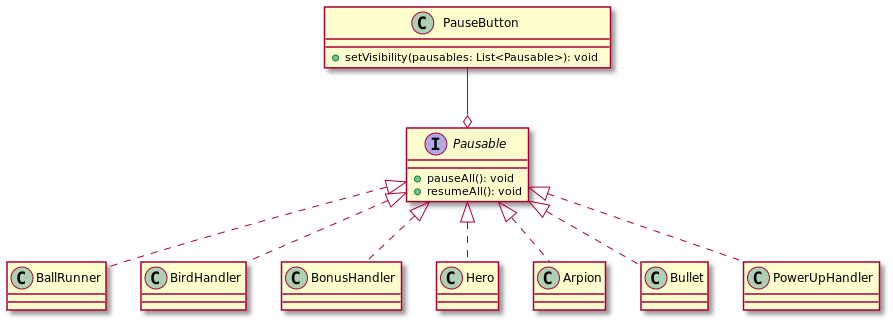
\includegraphics[width=15cm]{img/pause.png}
    \caption{Rappresentazione UML della gestione della pausa}
\end{figure}

\paragraph{Problema:} Il gioco deve supportare la pausa di oggetti multipli. Durante lo sviluppo ci siamo accorti che la funzione di pausa richiamava le stesse funzioni per tutti gli oggetti.

\paragraph{Soluzione:} Dato che i vari oggetti devono essere chiamati da un gestore della pausa, si è deciso di racchiudere questi oggetti dietro l’interfaccia \texttt{Pausable}. In questo modo è possibile, per il gestore, chiamare una funzione di pausa, ed una di avvio, su una lista di \texttt{Pausable} e quindi senza ripetizioni di codice.

\newpage
\subsubsection{HUD dinamico}
\begin{figure}[H]
    \centering
    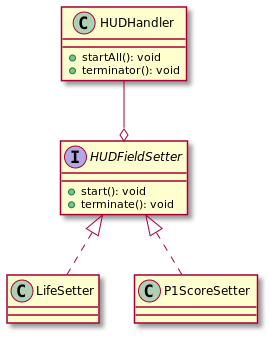
\includegraphics[width=6cm]{img/hud.png}
    \caption{Rappresentazione UML della gestione dell'HUD dinamico}
\end{figure}

\paragraph{Problema:} Il campo \texttt{Score} dell’HUD deve aggiornarsi quando il punteggio viene incrementato, similmente le vite.

\paragraph{Soluzione:} Sono state create due classi, chiamate da un gestore dedicato, improntate alla visualizzazione dello stato delle variabili in questione. Queste classi, inoltre, sono state racchiuse dentro l’interfaccia \texttt{HUDFieldSetter} in quanto utilizzano gli stessi metodi. Quando lo stato delle variabili cambia, i campi interessati dell’HUD vengono così aggiornati. 

\newpage
\subsubsection{Scelta di una direzione unica fino alla morte dell'uccello}
\begin{figure}[H]
    \centering{}
    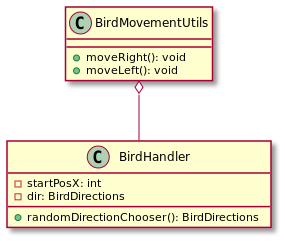
\includegraphics[width=7cm]{img/direct.png}
    \caption{Rappresentazione UML della gestione della scelta di una direzione}
\end{figure}

\paragraph{Problema:} La direzione dell’uccello viene generata casualmente, ma una volta generata non deve cambiare in base alla sua posizione fino alla fine del suo ciclo di vita.

\paragraph{Soluzione:} Durante l'implementazione delle funzioni di movimento abbiamo notato che la direzione dell'uccello cambiava in base alla sua posizione. È stata creata una classe \texttt{BirdHandler} la quale gestisce il ciclo di vita dell’uccello, compresa la creazione e la distruzione. Alla creazione viene definita una posizione iniziale decisa dalla direzione precedentemente generata. In base a questa, viene chiamato un metodo esterno dedicato al movimento dell’uccello nella direzione desiderata, in questo modo la direzione non potrà cambiare in base alla posizione.

\newpage
\subsubsection{Muovere l’uccello in base alla direzione scelta}
\begin{figure}[H]
    \centering{}
    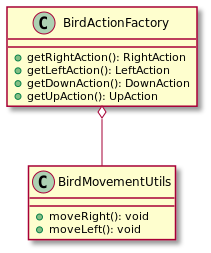
\includegraphics[width=5cm]{img/actionfact.png}
    \caption{Rappresentazione UML della gestione del movimento dell'uccello}
    \label{fig:my_label}
\end{figure}

\paragraph{Problema:} L’uccello, ad ogni movimento, deve cambiare posizione in base alla direzione generata randomicamente in precedenza.

\paragraph{Soluzione:} È stata creata una factory di cambio posizione dell’uccello in modo che, per ogni cambio posizione, venga chiamata uno dei metodi di movimento. Grazie a questo il codice è piú pulito.

\newpage
\subsection{Luca Rapolla}
\subsubsection{Portabilita' del personaggio principale (e della sua relativa arma) su un nuovo motore grafico}
\begin{figure}[H]
    \centering{}
    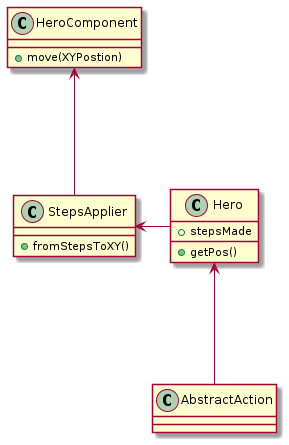
\includegraphics[width=7cm]{img/Actor.png}
    \caption{Rappresentazione UML della divisione tra Model e Visual}
    \end{figure}
    
\paragraph{Problema:}Il personaggio principale ha bisogno di muoversi all'interno di uno spazio il quale è determinato dal motore grafico che è possibile cambiare in base alle necessitá.

\paragraph{Soluzione:}Il personaggio principale e la sua arma sono divisi in \emph{Hero}, \emph{HeroComponent} ed \emph{Arpion}, \emph{ArpionComponent}. Sia \emph{Hero} che \emph{Arpion} mantengono le loro posizione assolute a prescindere dalle dimensioni della finestra di gioco e dal motore grafico usato.
Nel momento in cui si necessita di mettere in relazione le due entitá si usa un convertitore \emph{StepsConverter} che converte i passi fatti da \emph{Hero} in una posizione all'interno della finestra. Stessa cosa vale per \emph{Arpion} il quale, per salire verso l'alto, esegue un determinato numero di passi verso l'alto.

\newpage
\subsubsection{Eseguire azioni tramite la pressione di tasti (\emph{KeyBindings})}
\begin{figure}[H]
    \centering{}
    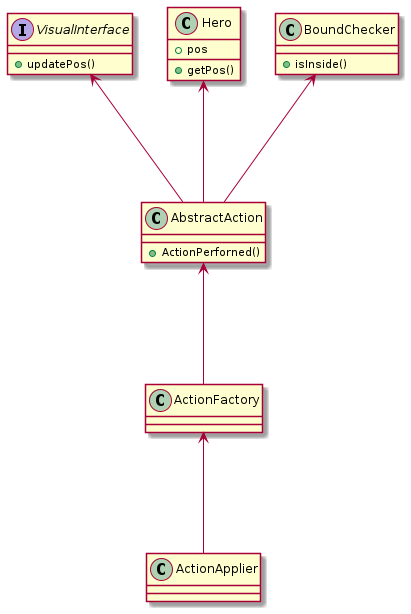
\includegraphics[width=10cm]{img/KeyBindings3.png}
    \caption{Rappresentazione UML del processo di avvenuta azione dopo la pressione di uno specifico tasto}
    \end{figure}

\paragraph{Problema:}Il giocatore deve poter comandare il personaggio principale tramite input da tastiera.

\newpage
\paragraph{Soluzione:}Per rendere il personaggio principale meno dipendente possibile dall'interfaccia di gioco si e' deciso di creare un sistema il quale collegando i tasti di gioco al pannello, questi richiamano semplici azioni che avranno effetto direttamente sulle caratteristiche del personaggio principale, al quale si chiede solo di cambiare i suoi attributi.(e.g. Volendo fare un passo verso sinistra, viene prima ricavata la posizione assoluta del personaggio principale da \emph{Hero} tramite \emph{StepsApplier}, in seguito viene fatto un controllo sulla prossima posizione in cui il personaggio principale dovra' spostarsi, se il controllo passa viene aggiornato \emph{Hero} e di conseguenza \emph{HeroComponent}.

\newpage
\subsubsection{Collisione del personaggio principale con un'entità ostile}
\begin{figure}[H]
    \centering{}
    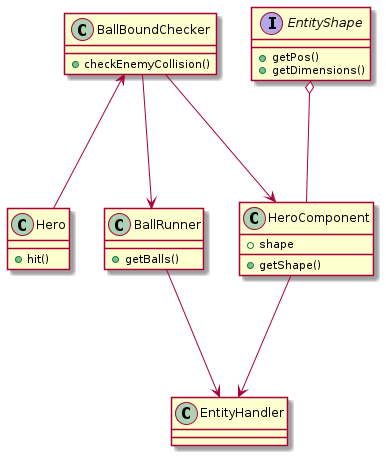
\includegraphics[width=7cm]{img/Collision.png}
    \caption{Rappresentazione UML del processo di rilevamento di una collisione ed  applicazione degli effetti relativi all'evento}
    \end{figure}
    
\paragraph{Problema:} Gestire l'evento di una collisione tra entità ed apllicarne gli effetti agli attori coinvolti.

\paragraph{Soluzione:} La riflessione di \emph{Hero} sulla finestra di gioco, ovvero \emph{HeroComponent}, utilizza un'interfaccia \emph{EntityShape} la quale tiene traccia delle dimensioni e della posizione di un'entità nello spazio.
Utilizzando un controller, il cui unico scopo è controllare le possibili collisioni tra le entità, si mette in relazione la \emph{Shape} del personaggio principale con la \emph{Shape} delle sfere. In caso di avvenuta collisione, si comunica l'evento ad \emph{Hero} il quale procederà a diminuire le vite disponibili e procederà a far duplicare la sfera che ha colpito il personaggio principale. La gestione dell'evento è equivalente nel caso si collida con l'entità uccello, l'unica differenza è che il nemico muore invece che duplicarsi.

\newpage
\subsubsection{Armi del personaggio principale}
    \begin{figure}[H]
    \centering
    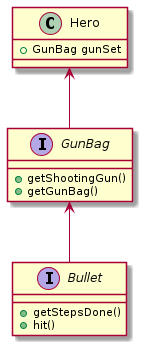
\includegraphics[height=7cm]{img/gunSet2.png}
    \caption{Rappresentazione UML della modellizzazione dell'arma data in dotazione al personaggio principale}
\end{figure}

\paragraph{Problema:} Assegnare al personaggio un arma capace di sparare diversi proiettili.

\paragraph{Soluzione:} Il personaggio principale e' dotato di un'arma \emph{GunBag} la quale puo' sparare dei proiettili, \emph{Bullet}. Il punto forte di questa progettazione e' l'alto potenziale di estendibilita' delle interfacce \emph{Bullet} e \emph{GunBag}, in questo modo e' possibile assegnare al personaggio principale un altra tipologia d'arma semplicemente implementando le interfacce sopra citate. L'unico punto debole di questa implementazione e' l'utilizzo di una \texttt{enum} per modellizzare le tipologie dei \emph{powerups} il che rende \emph{Arpion} non estendibile.

\newpage
\subsection{Ezmiron Deniuku}
\subsubsection{Input Utente}
    \begin{figure}[H]
    \centering
    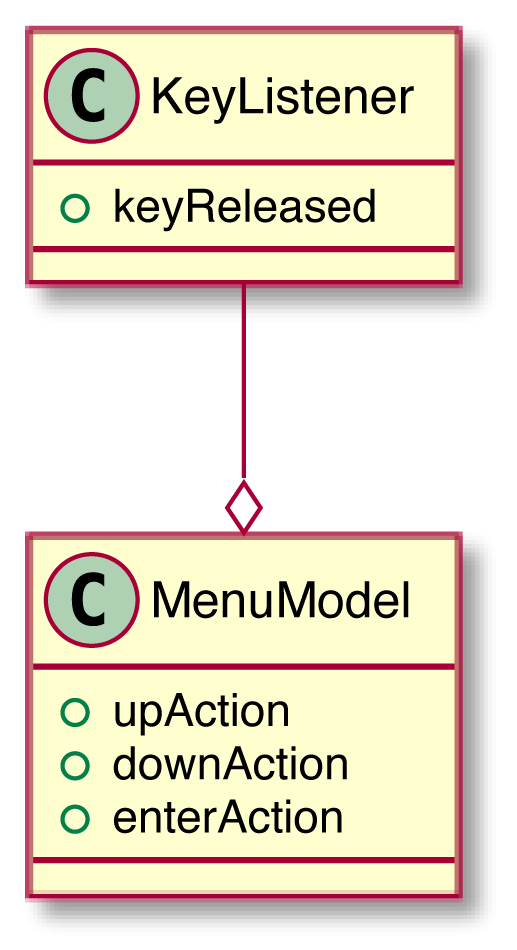
\includegraphics[height=7cm]{img/ez/2.png}
\end{figure}

\paragraph{Problema:} la classe \emph{MenuModel} deve riuscire a prendere in input i tasti premuti dall’utente.

\paragraph{Soluzione:} \emph{MenuModel} estende \emph{KeyListener} di cui eredità il metedo astratto keyReleased e sviluppa i suoi metodi.

\subsubsection{Etichette Dinamiche}
\paragraph{Problema:} necessità di avere delle etichette dinamiche per far capire quale voce è selezionata

\paragraph{Soluzione:} utilizzo della classe \emph{MenuLabel} che permette di settare colori, dimensioni, testi e rendere le scritte dinamiche tramite il metodo \texttt{switchBlink()}.
Gli altri metodi servono per realizzare etichette generiche come “PANG”

\subsubsection{Visualizzazione di caratteri digitati}
    \begin{figure}[H]
    \centering
    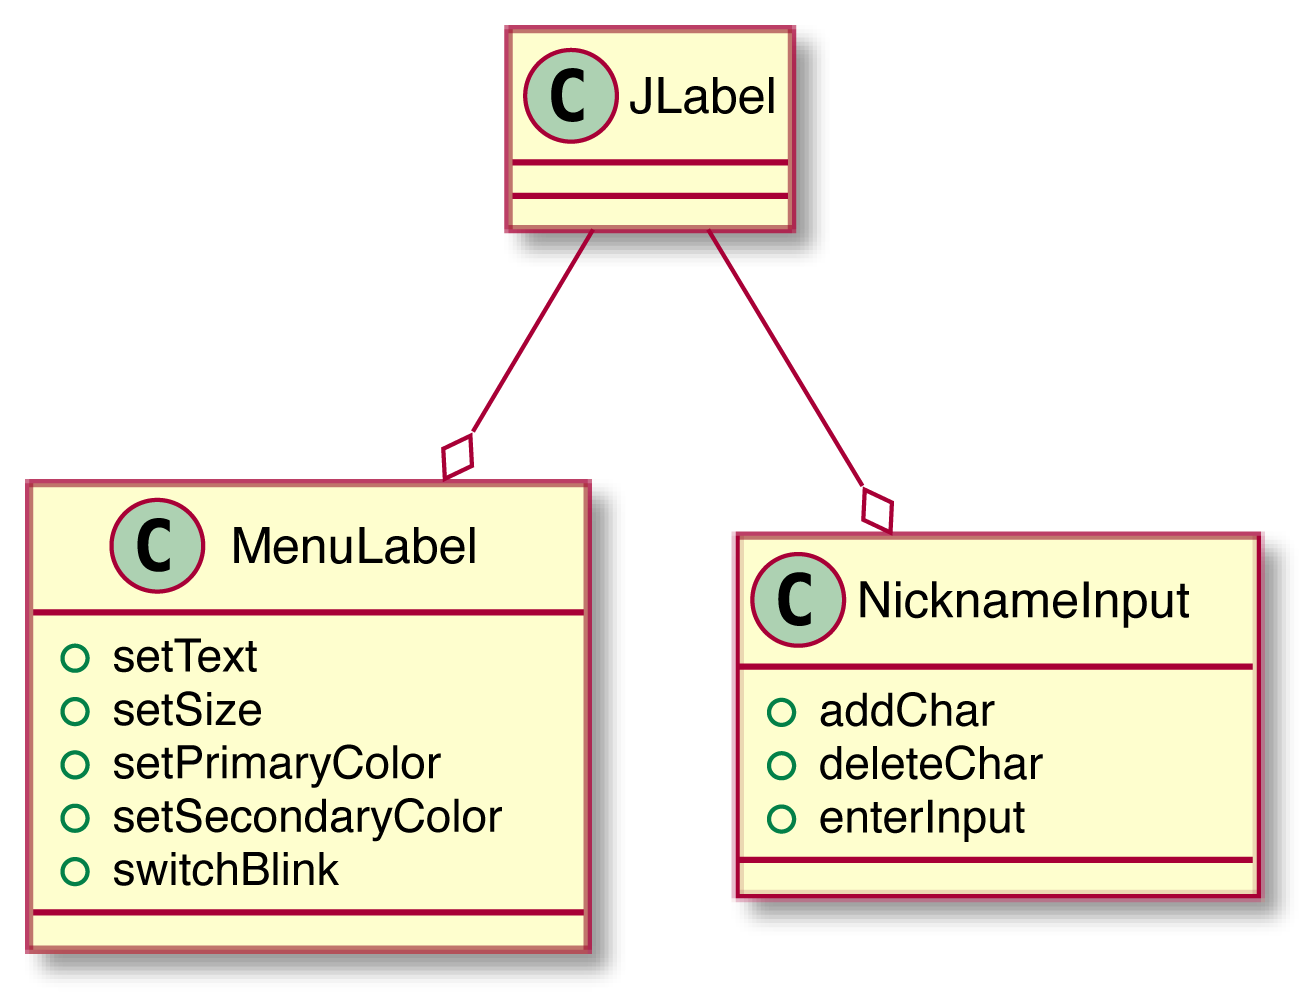
\includegraphics[height=7cm]{img/ez/3.png}
\end{figure}
\paragraph{Problema:} avere un modo di far visualizzare i caratteri che l’utente inserisce per il nome

\paragraph{Soluzione:} utilizzo \emph{NicknameInput} per creare l’etichetta dell’inserimento nel nome (“MARCO12”) che tramite \texttt{deleteChar()} o \texttt{addChar()} riesce a aggiornare di volta in volta.
Il metodo \texttt{enterInput()} servirà al momento del lancio del gioco. 

\subsubsection{Menu Interattivo}
    \begin{figure}[H]
    \centering
    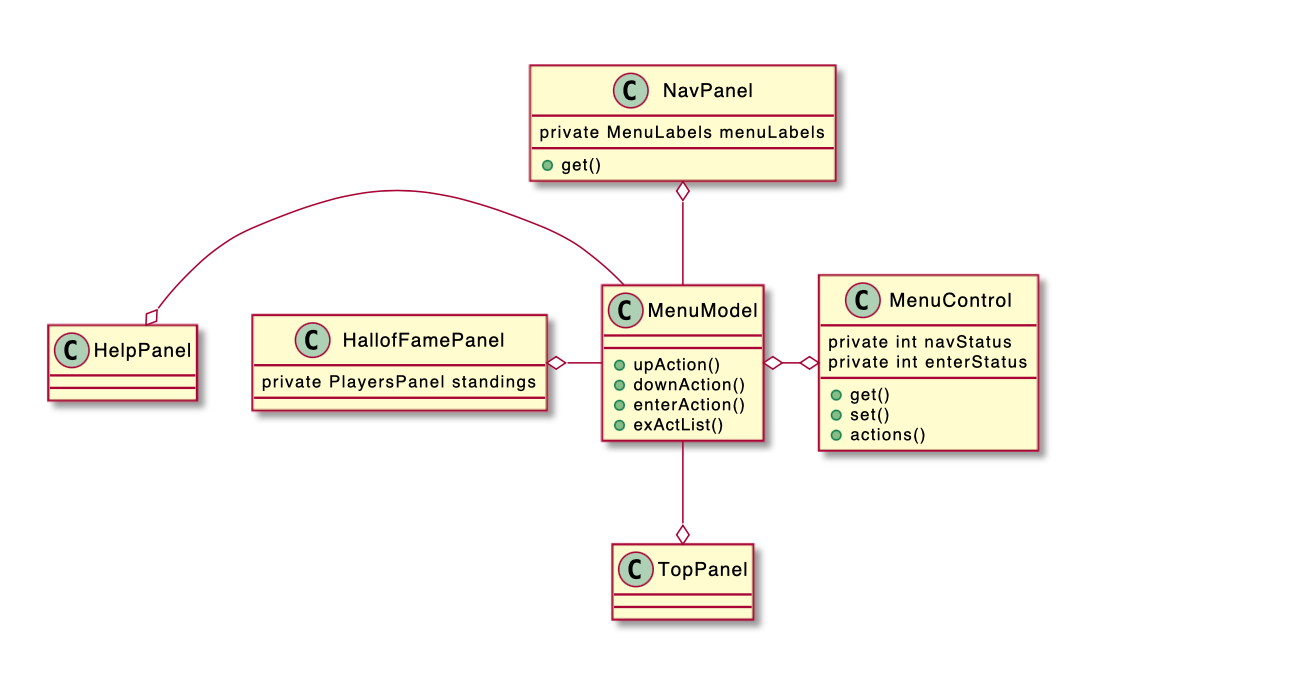
\includegraphics[height=7cm]{img/ez/5.png}
\end{figure}
\paragraph{Problema:} cambiare i pannelli in base alla propria selezione.
e.g.se l’utente seleziona la voce “HALL OF FAME”, visualizzare la hall of fame del gioco.
\paragraph{Soluzione:} MenuModel prende gli input dell’utente e tramite i suoi metodi \texttt{upAction()}, \texttt{downAction()}, \texttt{enterAction()} li manda a \emph{MenuControll}, la quale tiene conto di tutti gli input già avvenuti(tramite \emph{navStatus} e \emph{enterStatus}) ed elabora in seguito una nuova azione da eseguire e la restituisce a \emph{MenuModel}, che tramite \texttt{exActList()} agisce sulla gui andando a modificare i componenti di questa(le varie classi Panel).

\subsubsection{Salvataggio su file della \emph{Leaderboard}}
    \begin{figure}[H]
    \centering
    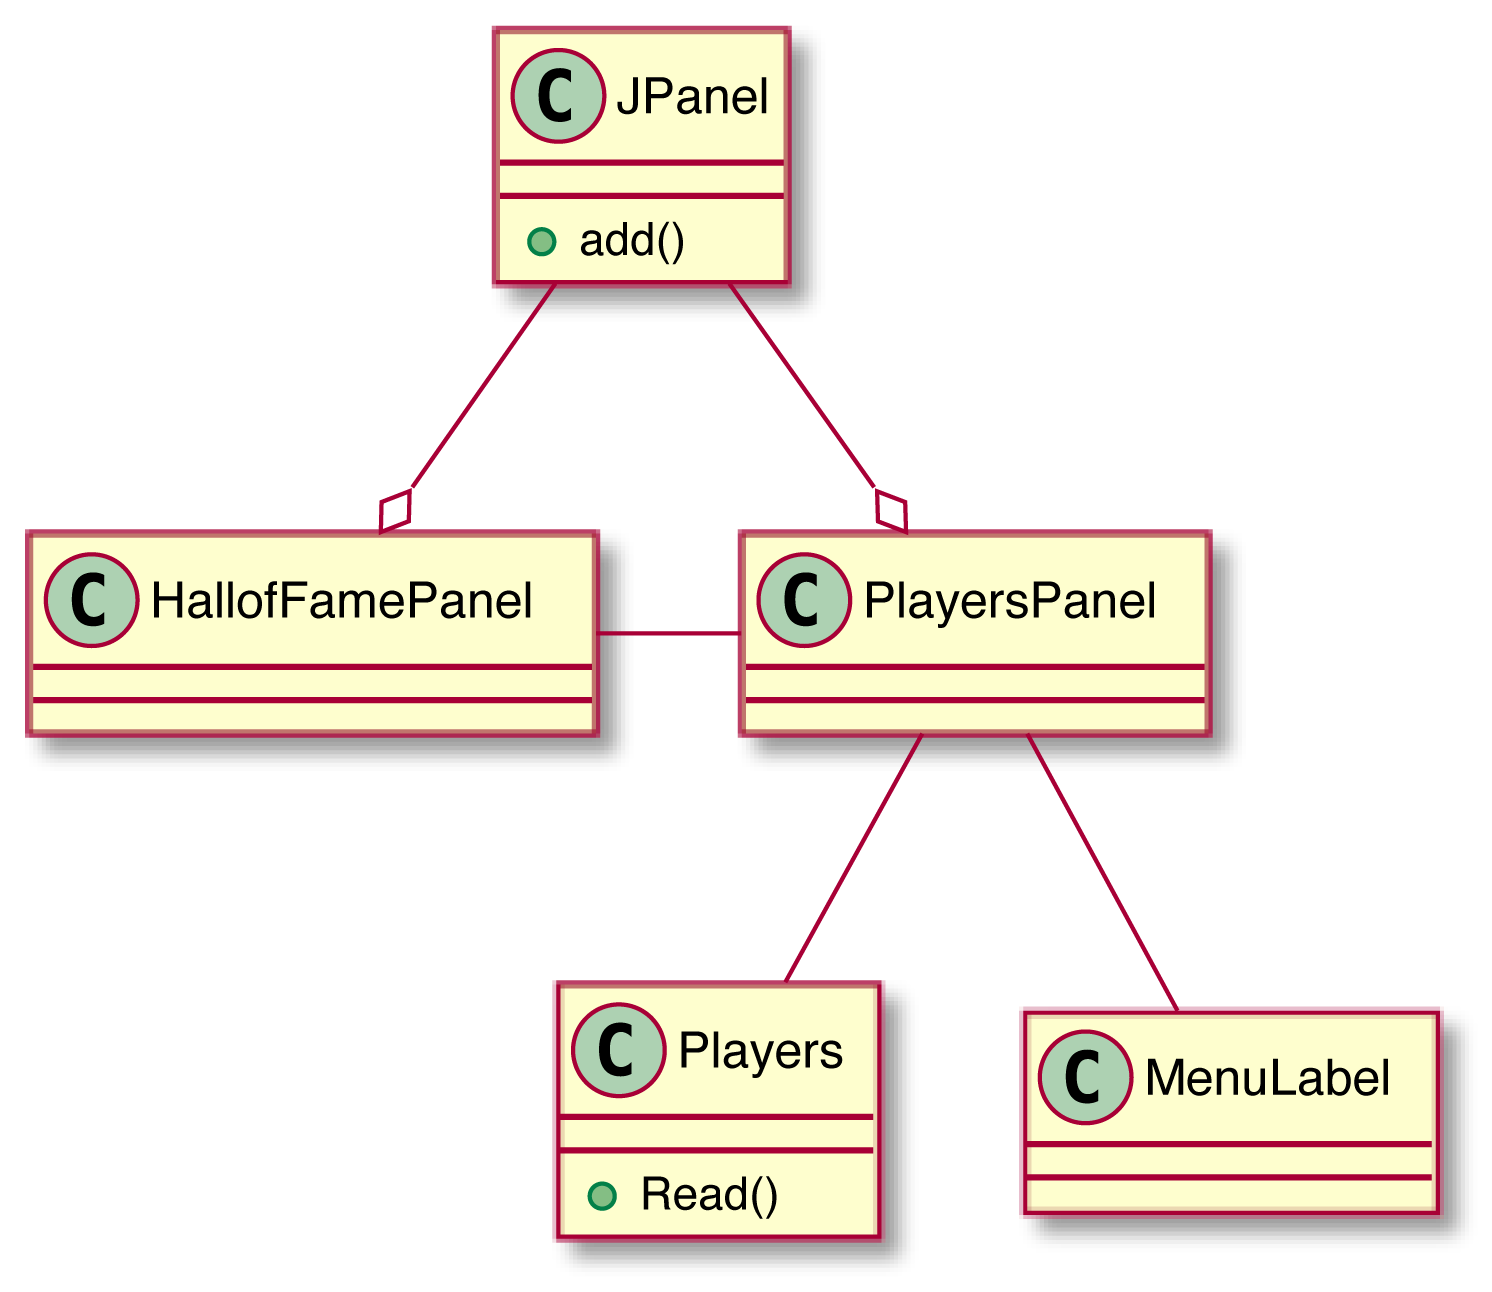
\includegraphics[height=7cm]{img/ez/6.png}
\end{figure}
\paragraph{Problema:} Riuscire a creare il panello con la hall of fame con tutti i giocatori che si riescono a estrarre dal metodo \texttt{Read()} della classe \emph{Players}.
\paragraph{Soluzione:}La classe \emph{HallOfFamePanel}  estende \emph{JPanel} e col suo metodo \texttt{add()} aggiunge a sé PlayersPanel che anche essa ha esteso \emph{JPanel} ed a sua volta ha aggiunto i dati dei giocatori tramite il metodo \texttt{} sotto forma di \emph{MenuLabel}.

\subsubsection{Avvio sessione di gioco}
    \begin{figure}[H]
    \centering
    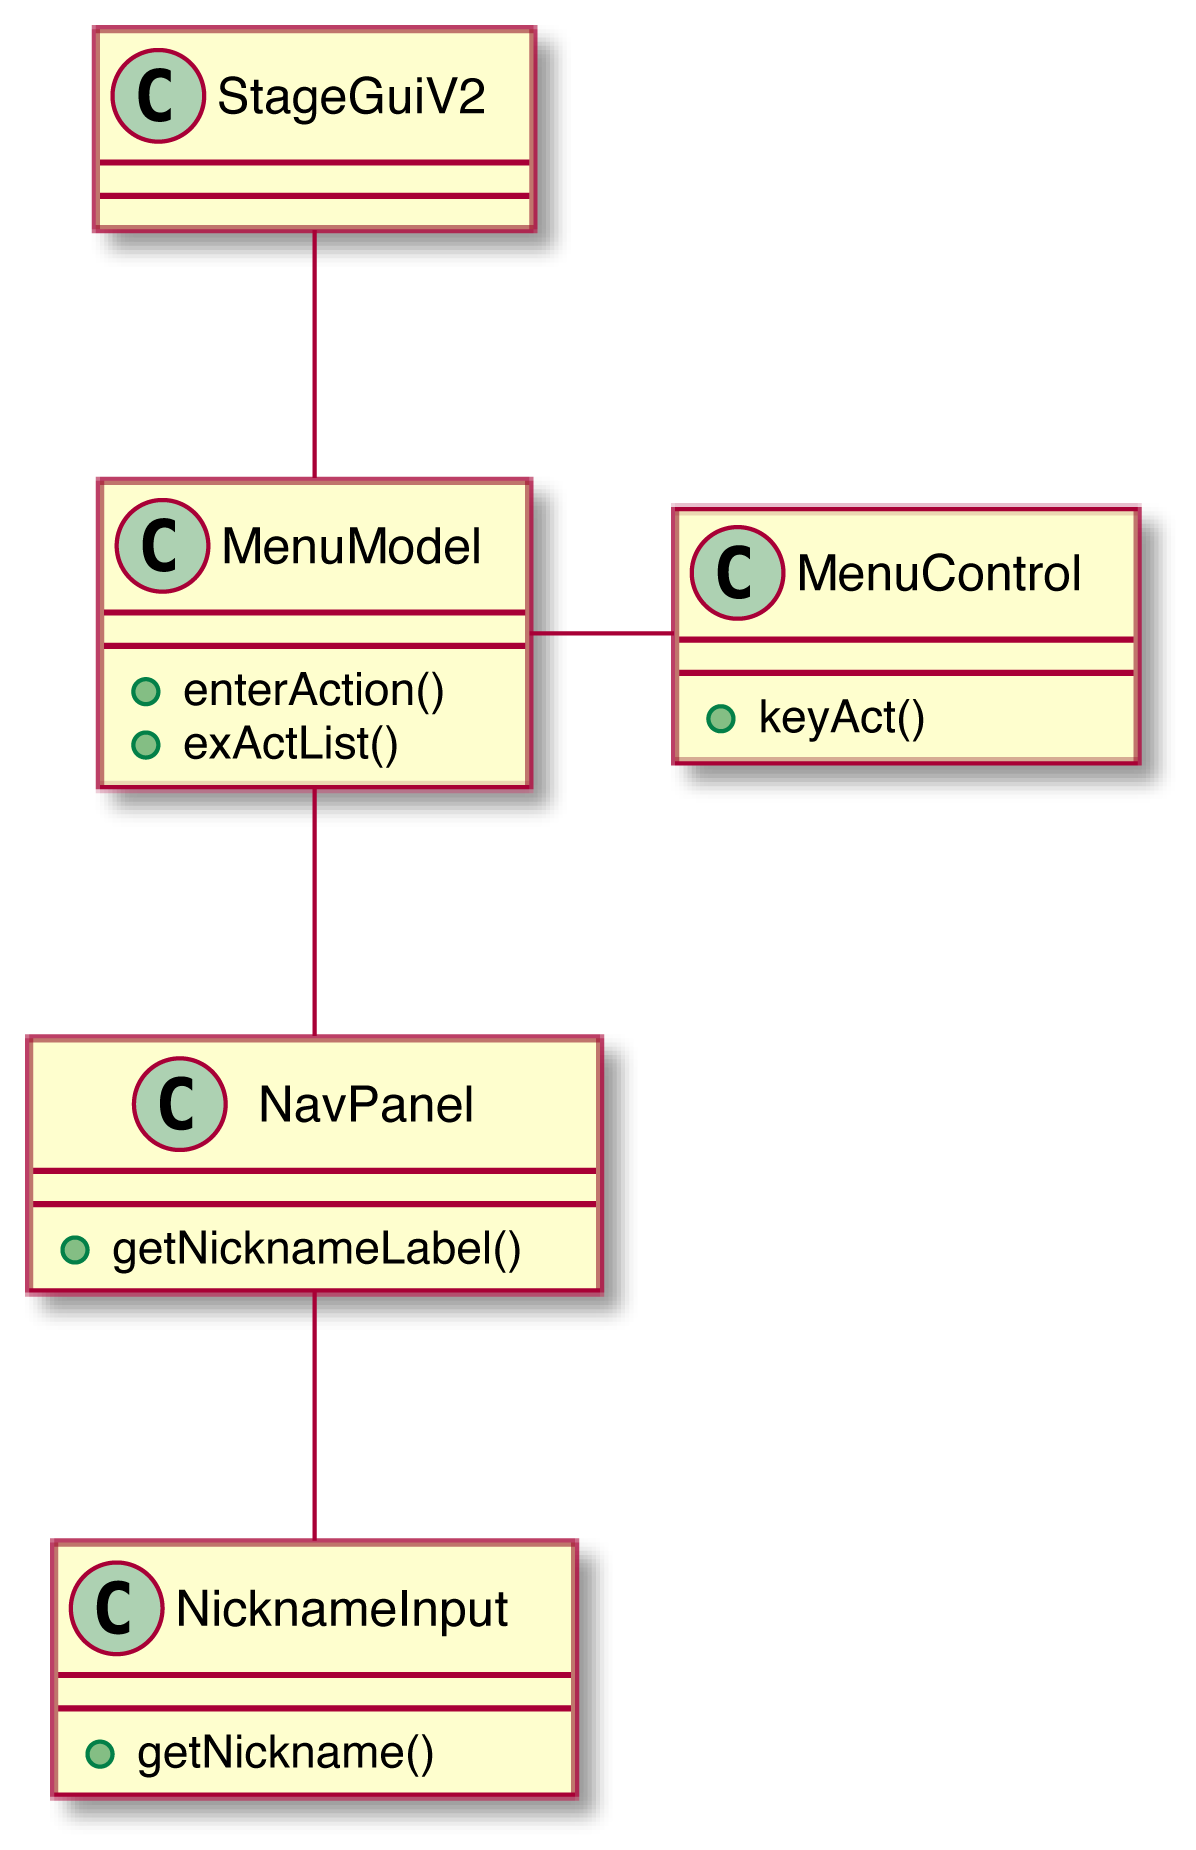
\includegraphics[height=7cm]{img/ez/7.png}
\end{figure}
\paragraph{Problema:} avviare il gioco quando l’utente inserisce il nickname e preme ENTER
\paragraph{Soluzione:} MenuModel riceve l’input dall’utente e tramire \texttt{enterAction()} lo manda a \emph{MenuControl}, 
quest’ultimo elabora l’input e col metedo \emph{keyAct} lo manda a \emph{MenuModel} che col metodo \texttt{exActList()} avvia \texttt{StageGuiV2} che si prende come parametro un \emph{Player} che viene generato \\(\texttt{NavPanel.getNicknameLabel().getNickname()}) sul momento prendendo il nome che l’utente aveva scritto fino a quel momento.

\subsubsection{Schermata di Fine Gioco e Salvataggio}
\begin{figure}[H]
    \centering
    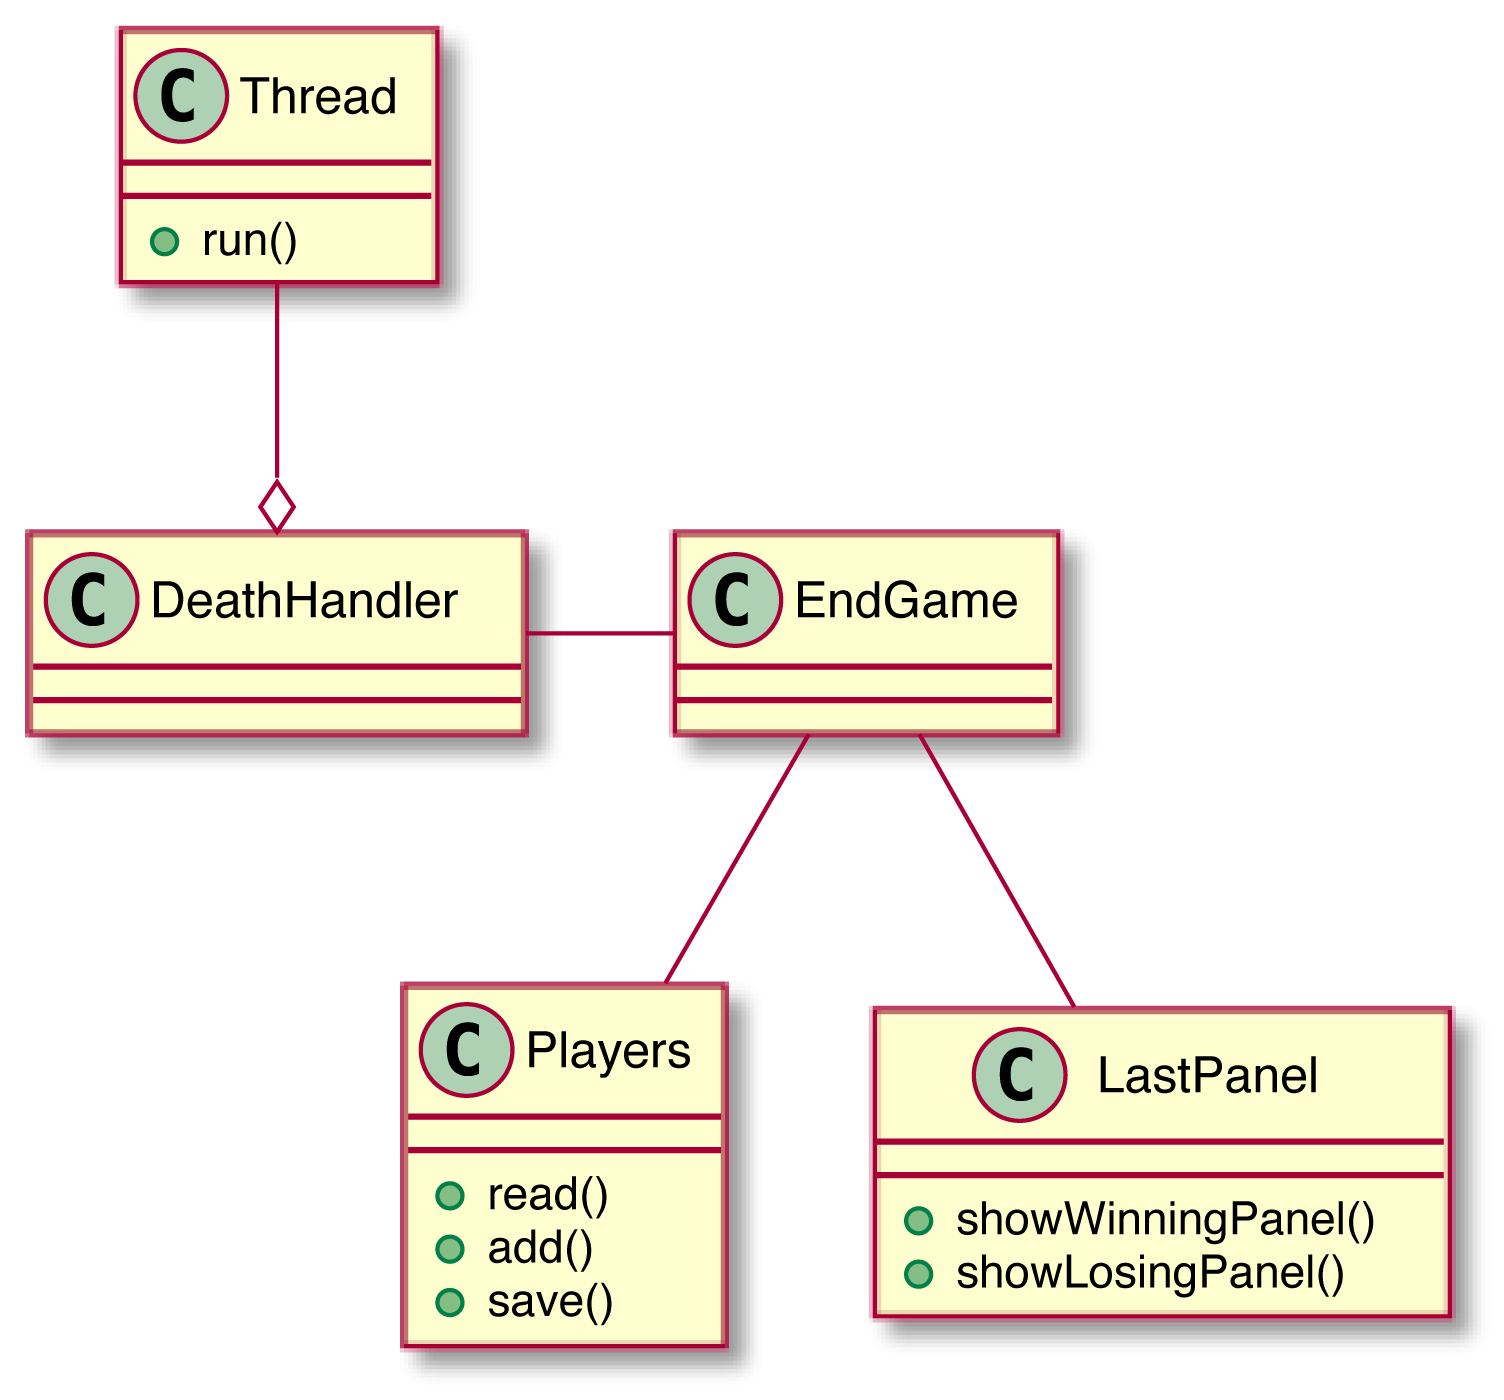
\includegraphics[height=7cm]{img/ez/8.png}
\end{figure}
\paragraph{Problema:} salvare i dati del giocatore in caso di vittoria e mostrare il pannello finale 
\paragraph{Soluzione:}  La classe DeathHandler che estende Thread verifica nel metodo \texttt{run()} lo stato di vittoria o sconfitta e passa l’informazione a EndGame che in base a questo chiama i metodi di LastPanel facendo visualizzare il pannello finale.
In caso di vittoria EndGame chiama i metodi di Players per aggiungere le stastische dell’ultimo giocatore e salvarle in caso di score rientrante in top 10.


\chapter{Sviluppo}
\section{Testing Automatizzato}

Il testing è stato svolto principalmente in maniera "visiva", ovvero che in base al comportamento di un entità, abbiamo stabilito se il funzionamento era corretto o meno. 

Il testing non è avvenuto in modo "automatico". Per le sfere, il testing è avvenuto attraverso l'interfaccia grafica e specialmente in fase iniziale, è stato necessario verificare che le formule utilizzate per emulare il moto parabolico della sfera avessero un riscontro visivo. Sempre per quest'ultimo motivo, i test riguardo la duplicazione e lo stop delle sfere sono sempre avvenuti attraverso interfaccia grafica e un pannello di controllo con dei bottoni, in modo tale da verificare il relativo effetto. Riguardo al pannello di controllo, nelle versioni iniziali era stato inserito nell'Action Listener dei bottoni, l'istanziazione del PowerUp Freeze e Bomb, ma con l'aggiornamento delle classi dei powerUp quei test sono risultati obsoleti (ora sono chiamati direttamente i metodi \emph{Duplicate} e \emph{Pause}). Allo stesso modo "visivo", sono avvenuti i test riguardo a tutte le entità che possono collidere tra di loro, in particolare: sfere-arpioni-eroe, uccello-arpioni-eroe ed eroe con bonus e powerUp. 

Per quanto riguarda il testing del corretto funzionamento dell’uccello è stato necessario tenere il testing manuale in quanto la direzione iniziale è randomica e in quanto quando colpisce l’Hero non deve scomparire mentre quando viene colpito da un arpione deve essere distrutto. È stato creato un frame di test apposito.

Per quanto riguarda il personaggio principale, sono stati svolti test principalmente in maniera "visiva" seguendo passo passo lo sviluppo del personaggio e della sua arma. I pirmi test svolti erano effettuati sulla corretta gestione dei movimenti comandati da \emph{input} da tastiera. Con l'aggiunta dei \emph{powerups} e dell'Arpione, e' stato costruito un controller ad hoc il quale agisce direttamente sulle caratteristiche degli attori in gioco in modo da simulare gli effetti dei \emph{powerups}.
Per quanto riguarda le interazioni con gli altri attori (Uccello e Sfere) sono stati usati dei \emph{log} appositi in grado di farci capire il modo in cui gli eventi si manifestavano.

Per quanto riguarda il testing relativo alla \emph{Hall of Fame}, si e' creata una finta entita' \texttt{Player} in modo da testare l'avvenuto salvataggio.

\section{Metodologia di lavoro}
\subsubsection{Michele Montesi}
\begin{itemize}
    \item Creazione dell’uccello come nemico aggiuntivo all’interno del gioco.
    \item Creazione dello stage di gioco completo di HUD dinamico (spiegato nel capitolo precedente). 
    \item Creazione di utility di sistema come \emph{MainImagesLoader} e \emph{MainFontLoader}, ovvero dei loader generici usati poi da loader più specifici.
    \item Creazione di utility di sistema per acquisire altezza e larghezza dello schermo principale.
    \item Creazione del menu di pausa e del suo funzionamento. Assieme a questo viene associata una utility che permette di uscire dal gioco con la pressione di un tasto.
\end{itemize}

Le parti di codice sono state sviluppate prima come stand-alone objects in modo da poter eseguire testing sufficienti. Una volta pronte sono state integrate con il resto del codice facendo il refactoring di tutto il necessario. Sicuramente quest’ultima parte è stata la piú difficile in quanto gestita male durante la fase di design.
L'utilizzo del \emph{DVCS} ha ricoperto un vantaggio fondamentale sia per quanto riguarda la collaborazione, sia per la cronologia del codice.
É stato usato su tre \emph{Branch} principali:
\begin{itemize}
    \item \texttt{Main}: \emph{Branch} principale, nel quale abbiamo pubblicato \emph{release} completamente funzionanti.
    \item \texttt{Feature}: \emph{Branch} di lavoro, qui e' stato effettuato la gran parte del lavoro sul progetto.
    \item \texttt{Feature Safe}: \emph{Branch} di lavoro sul quale poter testare parti di codice che possano temporaneamente sporcare il codice, in quanto questo \emph{Branch} é di test.
\end{itemize}


\subsubsection{Stefano Furi}
I seguenti aspetti sono quelli su cui è stato effettuato un lavoro individuale.
\begin{itemize}
    \item Progettazione, modellazione e implementazione delle sfere (package \texttt{ball}) sia negli aspetti di model e controller sia dal punto di vista di view.
    \item Progettazione di uno scheletro di controller in grado di gestire entità autonomamente, e riferire cambiamenti di stato alla view (vedere come riferimento classe \texttt{Visualiser} in \texttt{ball.gui}). 
    \item Progettazione dei \texttt{PowerUp} e i \texttt{Pickable}. 
    \item Implementazione dei \texttt{PowerUp} \texttt{Time Freeze} e \texttt{Bomb}.
    \item Implementazione del sotto-controller \texttt{PickableHandler}.
\end{itemize}
Aspetti su cui è stato effettuato un lavoro collettivo:
\begin{itemize}
    \item Progettazione e Sviluppo di \texttt{PowerUpEntity} e \texttt{PowerUpHandler} in collaborazione con Rapolla.
    \item Sviluppo su scheletro sopracitato della classe \texttt{EntityHandler} assieme a Rapolla e Montesi.
    \item Modellazione del concetto di \texttt{Pausable} assieme a Montesi.
\end{itemize}
Lo sviluppo della propria sottosezione (che comprendeva sia la parte di model sia di controller e view) è avvenuto completamente autonomamente. Il metodo di integrazione è stato quello di definire in fase di design, degli \emph{eventi} a cui il proprio dominio dovesse reagire (e.g. una Sfera che colpisce un arpione scaturisce una duplicazione). Nonostante questo, in fase di integrazione, abbiamo riscontrato difficoltà nel far comunicare le varie entità, ed è stato necessario un lavoro di riadattamento per quasi ognuna di esse. 

Per quanto riguarda l'utilizzo del DVCS, è stato usato localmente un branch denominato \emph{develop} per modificare/migliorare elementi costitutivi del modello mantenendo sempre una versione "funzionante" nel branch principale di sviluppo in caso di errori irrimediabili. Similmente, il branch remoto \emph{feature\_safe} è stato utilizzato da tutti i membri del gruppo durante la fase di integrazione, affinchè non venisse intaccata da possibili problemi la versione corrente funzionante nel branch principale di sviluppo \emph{feature}. Infine, nel branch \emph{main}, oltre alla preparazione iniziale della repository, sono state aggiunte solo versioni completamente funzionanti dell'applicazione.

\subsubsection{Luca Rapolla}
I seguenti aspetti sono stati svolti in maniera individuale.
\begin{itemize}
    \item Progettazione, modellizzazione ed implementazione del personaggio principale (package \texttt{PangGuy}) negli aspetti \emph{model}, \emph{view}, \emph{controller}.
    \item Progettazione, modellizzazione ed implementazione dei \emph{Keybindings} (package \texttt{PangGuy}).
    \item Progettazione e modellizzazione dei \emph{Bonus} (Package \texttt{Bonus}).
    \item Progettazione, modellizzazione ed implementazione dell'arma ed i suoi proiettili (Package \texttt{PangGuy}).
    \item Progettazione, modellizzazione ed implementazione dei \emph{powerups} \texttt{DoubleArpion} e \texttt{StickyArpion} (Package \texttt{PowerUp}).
\end{itemize}

Parti sviluppate in gruppo:
\begin{itemize}
    \item Progettazione e sviluppo di \emph{PowerupEntity} e \emph{PowerupHandler} con Furi.
    \item Progettazione e sviluppo di \emph{DeathHandler} con Deniku.
    \item Implementazione dei \emph{Bonus} con Deniku.
\end{itemize}

Lo sviluppo delle varie parti del codice e'stato svolto singolarmente. Causa l'inseperienza nel prendere parte in lavori di gruppo, abbiamo verificato, soprattutto in caso di unione del personaggio principale con le sfere, la difficolta' nel relazionare efficacemente le due parti in quanto abbiamo constatato di esserci impegnati piu' sulla praticita' di una classe che alla fusione con altre classi.

Per quanto riguarda l'utilizzo del \emph{DVCS}, e' stato usato su tre \emph{Branch} principali:
\begin{itemize}
    \item \texttt{Main}: \emph{Branch} principale, nel quale abbiamo pubblicato \emph{release} completamente funzionanti del gioco in modo da avere sempre una versione pronta e funzionante.
    \item \texttt{Feature}: \emph{Branch} di lavoro, qui e' stato effettuato la gran parte del lavoro sul progetto.
    \item \texttt{Feature Safe}: \emph{Branch} di lavoro secondario, usato principalmente in casi di grosse modifiche che avrebbero potuto influire negativamente sull'integrita' del progetto.
\end{itemize}

\subsubsection{Ezmiron Deniku}

\begin{itemize}
    \item 
\end{itemize}

Arrivando dalla programmazione ad oggetti fatta in \emph{C#}, ho dovuto reinventarmi completamente, e queste inizialmente lo ho fatto riguardando le slide delle lezione da me saltate poiché ero in \emph{Erasmus}, cercando di capire non solo questo nuovo linguaggio, ma anche cercando di unire a quanto ho imparato nella università ospitante. 

Il grosso del mio lavoro si basava sulla parte grafica, cosa da me esplicitamente richiesta in fase iniziale, poiché come dissi per email al prof. Viroli in lituania non mi avevo mai visto come lavorare a parti grafiche. Inizialmente ho cercato di prendere spunto dall’operato Michele Montesi che doveva creare il pannello basso nel gioco, ma ovviamente questo non è bastato poiché la mia gui doveva essere dinamica e quindi ho fatto qualche ricerca su stackoverflow e ho letto documentazioni di librerie come GridBagLayout e GridBagConstraints.

\section{Note di sviluppo}
\subsubsection{Michele Montesi}

\begin{itemize}
    \item Utilizzo di lambda nel metodo \emph{setVisibility()} di \texttt{pauseMenu.components.PauseButton}.
    \item Uso di \emph{\(Optional<BirdActor>\)} in \texttt{bird.controller.BirdHandler}.
    \item Uso di \emph{\(Optional<BirdShape>\)} in \texttt{bird.controller.BirdHandler}.
    \item Caching degli sprite per l’uccello in \texttt{bird.utilities.BirdPNGLoader}.
    \item \subsubsection{Risorse}
    \begin{itemize}
        \item Aggiungere componenti in una specifica posizione di un JPabel:
        \url{https://stackoverflow.com/questions/2510159/can-i-add-a-component-to-a-specific-grid-cell-when-a-gridlayout-is-used}
        \item Rimuovere alone attorno ad uno sprite: \url{https://stackoverflow.com/questions/71797654/bufferedimage-drawn-on-jlabel-doesn-keep-transparent-background}
    \end{itemize}
\end{itemize}

\subsubsection{Stefano Furi}
\begin{itemize}
    \item Utilizzo dell'interfaccia funzionale \texttt{Function} in \texttt{ball.physics.Trajectory} nel metodo \texttt{relativeSpeed}.
    \item Utilizzo di generici nella classe astratta \texttt{utilities.Pos2D}.
    \item Utilizzo di Stream in \texttt{EntityHandler} e \texttt{PickableHandler} nei motodi \texttt{getPausable()} e un simile utilizzo è presente in \texttt{Controller}.
\end{itemize}
Porzioni di codice reperite in rete:
\begin{itemize}
    \item Moto del Proiettile:
    \url{https://www.101computing.net/projectile-motion-formula/}
    \item Snippet intersezione tra Rettangolo e Cerchio:  \url{https://stackoverflow.com/questions/401847/circle-rectangle-collision-detection-intersection}
    \item Snippet sovrapposizione tra Rettangoli:
    \url{https://stackoverflow.com/questions/23302698/java-check-if-two-rectangles-overlap-at-any-point}
\end{itemize}

\subsubsection{Luca Rapolla}
\begin{itemize}
    \item Uso di Optional nello sviluppo dell'arma in \texttt{pangGuy.modularGun}, in \texttt{bonus.BonusHandler.java}, in \texttt{powerup.PowerUpHandler.java}
    \item Uso di \emph{Generics} in \texttt{FullPair.java}
    \item Uso di una Factory in \texttt{panguy.actions.ActionFactory.java}
\end{itemize}

Porzioni di codice reperite in rete:
\begin{itemize}
    \item KeyBindings (Ho preso solo spunto per la funzione da usare, il codice in se era di male fattura): \url{https://www.youtube.com/watch?v=IyfB0u9g2x0&ab_channel=BroCode}
\end{itemize}

\subsubsection{Ezmiron Deniku}
Quando andavo a salvare e leggere le prime volte cercavo di tenere un file di testo (“bestPlayersSaves.txt”) nella cartella delle risorse e per poi sovrascriverlo sempre lì.

Per cercare il filepath utilizzavo ClassLoader.getSystemResourceAsStream(), andando poi a scrivere con getResoursce(dandogli il classhpath), ed il tutto funzionava finchè si lanciava da eclipse, ma poi andando a lanciare da jar non funzionava.

Su siti come stackoverflow ho trovato che dovrebbe essere impossibile creare file all’interno di un jar.

Quindi ho ovviato al problema, con l’auito di Michele Montesi, andando a creare il file di salvataggio fuori dal jar nella cartella app del progetto.

\chapter{Commenti Finali}
\section{Autovalutazione e lavori futuri}
\subsubsection{Michele Montesi}
Le ore ricoperte sono bastate per completare le sezioni di progetto a me attribuite. Non é stato attribuito tempo sufficiente al design, il quale ha portato a diversi problemi nella rifattorizzazione di vari componenti con quelli dei colleghi. 

\subsubsection{Punti di forza}

\begin{itemize}
    \item Il menu e la funzione di pausa funzionano correttamente.
    \item L’HUD si aggiorna automaticamente.
    \item L’uccello si integra con l’ambiente di gioco senza creare conflitti di alcun tipo.
    \item Riuso del codice
\end{itemize}

\subsubsection{Punti di debolezza}
\begin{itemize}
    \item Lo stage non viene generato sempre in 16:9 ma prende le dimensioni in base all’altezza e alla larghezza dello schermo.
    \item Scarsa comunicazione nelle prime fasi, la quale ha causato riprogettazione e refattorizzazione del codice.
    \item Possibile utilizzo di troppi thread.
\end{itemize}

Il ruolo che ho ricoperto consiste nella creazione del nemico \texttt{Bird} e delle sue funzionalità, nonché alla creazione di varie utility di sistema per lo stage. È stato anche creato il menu e la funzione di pausa e di uscita dal gioco mentre in pausa. Mi sono sempre reso disponibile per controllare il codice dei miei colleghi ed aiutarli a risolvere eventuali problemi.

\subsubsection{Stefano Furi}
La sottoparte del modello dell'applicativo assegnata, è risultata sufficiente per ricoprire le ore di lavoro richieste dai docenti. La fase di progettazione individuale è stata più che altro funzionale (come gestire il tutto e integrarlo con gli altri elementi) e non è stato attribuito abbastanza tempo al design. Infatti, per porzioni più corpose come la sfera, non sono praticamente presenti \emph{design patterns} ma solo soluzioni più o meno efficaci in base al problema riscontrato. D'altro canto, per la modellazione dei PowerUp, è stata attribuita più attenzione al design, in quanto già in fase di analisi con i colleghi, venivano fuori molte problematiche legate alla proliferazione di istanze molto simili ma che differivano di poco nel comportamento. Riassumendo quindi:
\begin{itemize}
    \item PowerUp estendibili e molto riuso di codice.
    \item Diversi livelli di controllo e di astrazione per le sfere, rendendo comprensibile al client le funzioni e potenzialità delle sfere.
    \item Scorporamento del controller principale in sotto controller, in modo tale da delegare a ognuno di essi una sottoparte del dominio applicativo e rendere più semplice gestire eventuali errori.
\end{itemize}
D'altra parte, i punti di debolezza principali:
\begin{itemize}
    \item Insufficiente progettazione individuale del design.
    \item Scarsa considerazione degli aspetti necessari per l'integrazione di tutti i componenti del sistema, la quale ha causato molto lavoro di riprogettazione e adattamento.
    \item Possibile uso improprio delle funzionalità dei \texttt{Thread}.
    \item Poca considerazione delle performance. 
\end{itemize}
All'interno del gruppo di lavoro, in quanto avendo iniziato e "finito" per primo la parte di modello, mi sono reso disponibile nell'aiutare i miei compagni nell'interfacciamento delle loro classi con il controller principale. Inoltre, ho aiutato e collaborato con i miei colleghi nella creazione e corretta implementazione delle entità in grado di gestire l'integrazione di tutti gli elelemti del dominio (i sotto-controller) durante la fase finale di sviluppo.

\subsubsection{Luca Rapolla}
La sottoparte del software realizzata e' risultata sufficente sia in ambito di difficolta' che in ambito di tempo utilizzato per produrla rispetto alle ore di lavoro richieste.
Un punto molto forte del lavoro di gruppo, secondo il mio parere, e' stato quello di conoscerci tutti di persona, questo ha abbattuto la barriera dell'imbarazzo verso uno sconosciuto e ci ha dato la possibilita' di essere piu aperti e sinceri verso gli altri componenti del gruppo.
A mio avviso l'uso del \emph{DVCS} poteva essere perfezionato ma, essendo la prima esperienza "sul campo", comprendo i nostri limiti.
Per quanto riguarda il codice invece, posso delineare i seguenti lati positivi:
\begin{itemize}
    \item Il dialogo ben riuscito tra personaggio principale e le sue armi.
    \item La semplice assegnazione delle immagini dei \emph{Bonus} tramite i loro punti.
    \item Il dialogo tra le sfere e l'arpione.
\end{itemize}

Per quanto riguarda i lati negativi invece:
\begin{itemize}
    \item I troppi pochi \emph{powerups} creati.
    \item La richiesta modestamente alta di CPU causata dai Thread.
\end{itemize}

In futuro vorrei aggiungere piu armi al personaggio principale e creare piu' \emph{Powerups}.



\begin{appendices}
\chapter{Guida utente}
\subsubsection{Utilizzo della \emph{LeaderBoard}}
\begin{itemize}
    \item All'avvio del gioco viene controllato se il file di salvataggio della \emph{LeaderBoard} si trova nella stessa directory del JAR. Nel caso in cui non ci sia viene creato.
\end{itemize}

\subsubsection{Controlli}
\begin{itemize}
    \item \texttt{Frecce direzionali:} Movimento a destra e sinistra del personaggio principale.
    \item \texttt{Barra spaziatrice:} Utilizzo dell'arma attuale.
\end{itemize}


\chapter{Esercitazioni di laboratorio}
\subsubsection{Michele Montesi}

\begin{itemize}
    \item Laboratorio 05: \url{https://virtuale.unibo.it/mod/forum/discuss.php?d=87881#p138074}
    \item Laboratorio 06: \url{https://virtuale.unibo.it/mod/forum/discuss.php?d=87880#p138072}
    \item Laboratorio 07: \url{https://virtuale.unibo.it/mod/forum/discuss.php?d=88829#p138076}
    \item Laboratorio 08: \url{https://virtuale.unibo.it/mod/forum/discuss.php?d=89272#p138077}
    \item Laboratorio 09: \url{https://virtuale.unibo.it/mod/forum/discuss.php?d=90125#p138555}
\end{itemize}

\subsubsection{Stefano Furi}
\begin{itemize}
    \item Laboratorio 06:
    \url{https://virtuale.unibo.it/mod/forum/discuss.php?d=87880#p138782}
    \item Laboratorio 07:
    \url{https://virtuale.unibo.it/mod/forum/discuss.php?d=88829#p138781}
    \item Laboratorio 08:
    \url{https://virtuale.unibo.it/mod/forum/discuss.php?d=89272#p138780}
    \item Laboratorio 09:
    \url{https://virtuale.unibo.it/mod/forum/discuss.php?d=90125#p138779}
\end{itemize}

\subsubsection{Luca Rapolla}
\begin{itemize}
    \item Laboratorio 09:
    \url{https://virtuale.unibo.it/mod/forum/discuss.php?d=90125#p138405}
    \item Laboratorio 08:
    \url{https://virtuale.unibo.it/mod/forum/discuss.php?d=89272#p138048}
    \item Laboratorio 07:
    \url{https://virtuale.unibo.it/mod/forum/discuss.php?d=88829#p136506}
    \item Laboratorio 06:
    \url{https://virtuale.unibo.it/mod/forum/discuss.php?d=87880#p136596}
    \item Laboratorio 05:
    \url{https://virtuale.unibo.it/mod/forum/discuss.php?d=87881#p138042}
\end{itemize}

\end{appendices}

\end{document}